\documentclass[11pt,letter]{article}
\usepackage[top=1.00in, bottom=1.0in, left=1.1in, right=1.1in]{geometry}
\renewcommand{\baselinestretch}{1.1}
\usepackage[
singlelinecheck=false % <-- important
]{caption}
\usepackage{hyperref}%helps with the email address 
\usepackage{graphicx} %including pictures 

\def\labelitemi{--}
\parindent=0pt

\def\labelitemi{--}
\parindent=0pt

\newenvironment{smitemize}{
\begin{itemize}
  \setlength{\itemsep}{0pt}
  \setlength{\parskip}{0.8pt}
  \setlength{\parsep}{0pt}}
{\end{itemize}
}

\graphicspath{ {./protPhotos/} }% tell latex where to find photos 

\begin{document}

\bibliographystyle{/Users/Lizzie/Documents/EndnoteRelated/Bibtex/styles/besjournals}
\renewcommand{\refname}{\CHead{}}

\title{Protocol for Okanagan winegrape phenology \\ set-up and monitoring}
\date{ }
\maketitle
\tableofcontents



\section{Objectives}
We aim to characterize the phenology of seven of the most commonly planted winegrape varieties in vineyards throughout the Okanagan Valley in British Columbia. Our primary goal is to improve grower models of plant development with relation to climate. To this end, we will monitor a diversity of varieties that capture differences in phenology. We will record the phenology for selected vines for 2-3 growing seasons from budburst through the summer to veraison. We will also track fruit development through periodic Brix measurements after veraison.

\section{Set up Protocol}

\subsection{Sampling Population}
Varieties sampled: Merlot, Pinot noir, Chardonnay, Riesling, Sauvignon blanc, Syrah (Shiraz), Cabernet-Sauvignon \\
Arterra sites: McIntyre, Dark Horse, NK'MIP Cellars \\ %removed Whitetail 
Quails' Gate sites: Quails' Gate Estate vineyard, Mannhardt \\
% Sebastian Farms (Mission Hill) sites:

\subsection{Choosing Vines}

Using the maps and rootstock information provided, we chose the blocks with the following considerations in mind:
\begin{smitemize}
\item Sample all of our target varieties.
\item We chose blocks of different varieties near each other if possible to reduce walking distance/time. 
\item If a vineyard had multiple blocks of a variety and the blocks were different parts of the vineyard, we sampled one block in each general area to capture environmental variation within the site. If the blocks are close together, we chose to sample just one block.
\item If we sampled multiple blocks of a variety in a vineyard, we would usually sample 24 vines in each block rather than 36 to reduce time.
\item We preferentially chose blocks with common rootstocks - 3309, 101-14, S04 - in order to reduce effect of rootstock.
\item We avoided blocks with unknown clones or varieties and were able to avoid all of the self-rooted blocks except one (Dark Horse block G, the other Pinot noir block was recently planted).
\item When weather station locations were known, we chose rows or blocks near them.
\item Within blocks, we aimed to capture environmental variation in block, keeping in mind time needed to walk between location. Often this meant that we would sample at the bottom and top of block in the same rows if we flagged 24 plants. If we flagged 36, we would add a middle location in a different set of rows. 
\item We sampled 6 plants per row in each location. We aimed for plants to be next to each other but sometimes had to skip plants if they were too young or if they did not have a cordon with 2 spurs/cane with 2 buds. Such cases are marked in the Plant ID spreadsheet.
\item Flagged vines are at least 6 plants in from the end of the row so we avoid edge effects.
\item We always chose to sample two rows next to each other in each location so there were 12 plants (6 per row) in each location.
\item 36 or 24 vines were flagged per block.

\end{smitemize}

Tip for when selecting buds each year: If you are not flagging all the buds at once, flag the final bud/spur as this one will always be monitored. Doing this saves time because otherwise you may have to move the flag to another spur. We would recommend flagging with flagging tape all the buds at once to save time.\\

The location of each plant we monitor, as well as which side of the plant we chose to monitor, (see Choosing Buds below) is recorded in the \verb|plantsinfo.csv| file on the repo. \\

During the first season, some of the flagged vines were not producing enough clusters for bloom monitoring. Flags were transferred from these vines to other nearby vine by April Mahovlic and their location was recorded.

\subsection{Choosing Buds}


\begin{figure}
  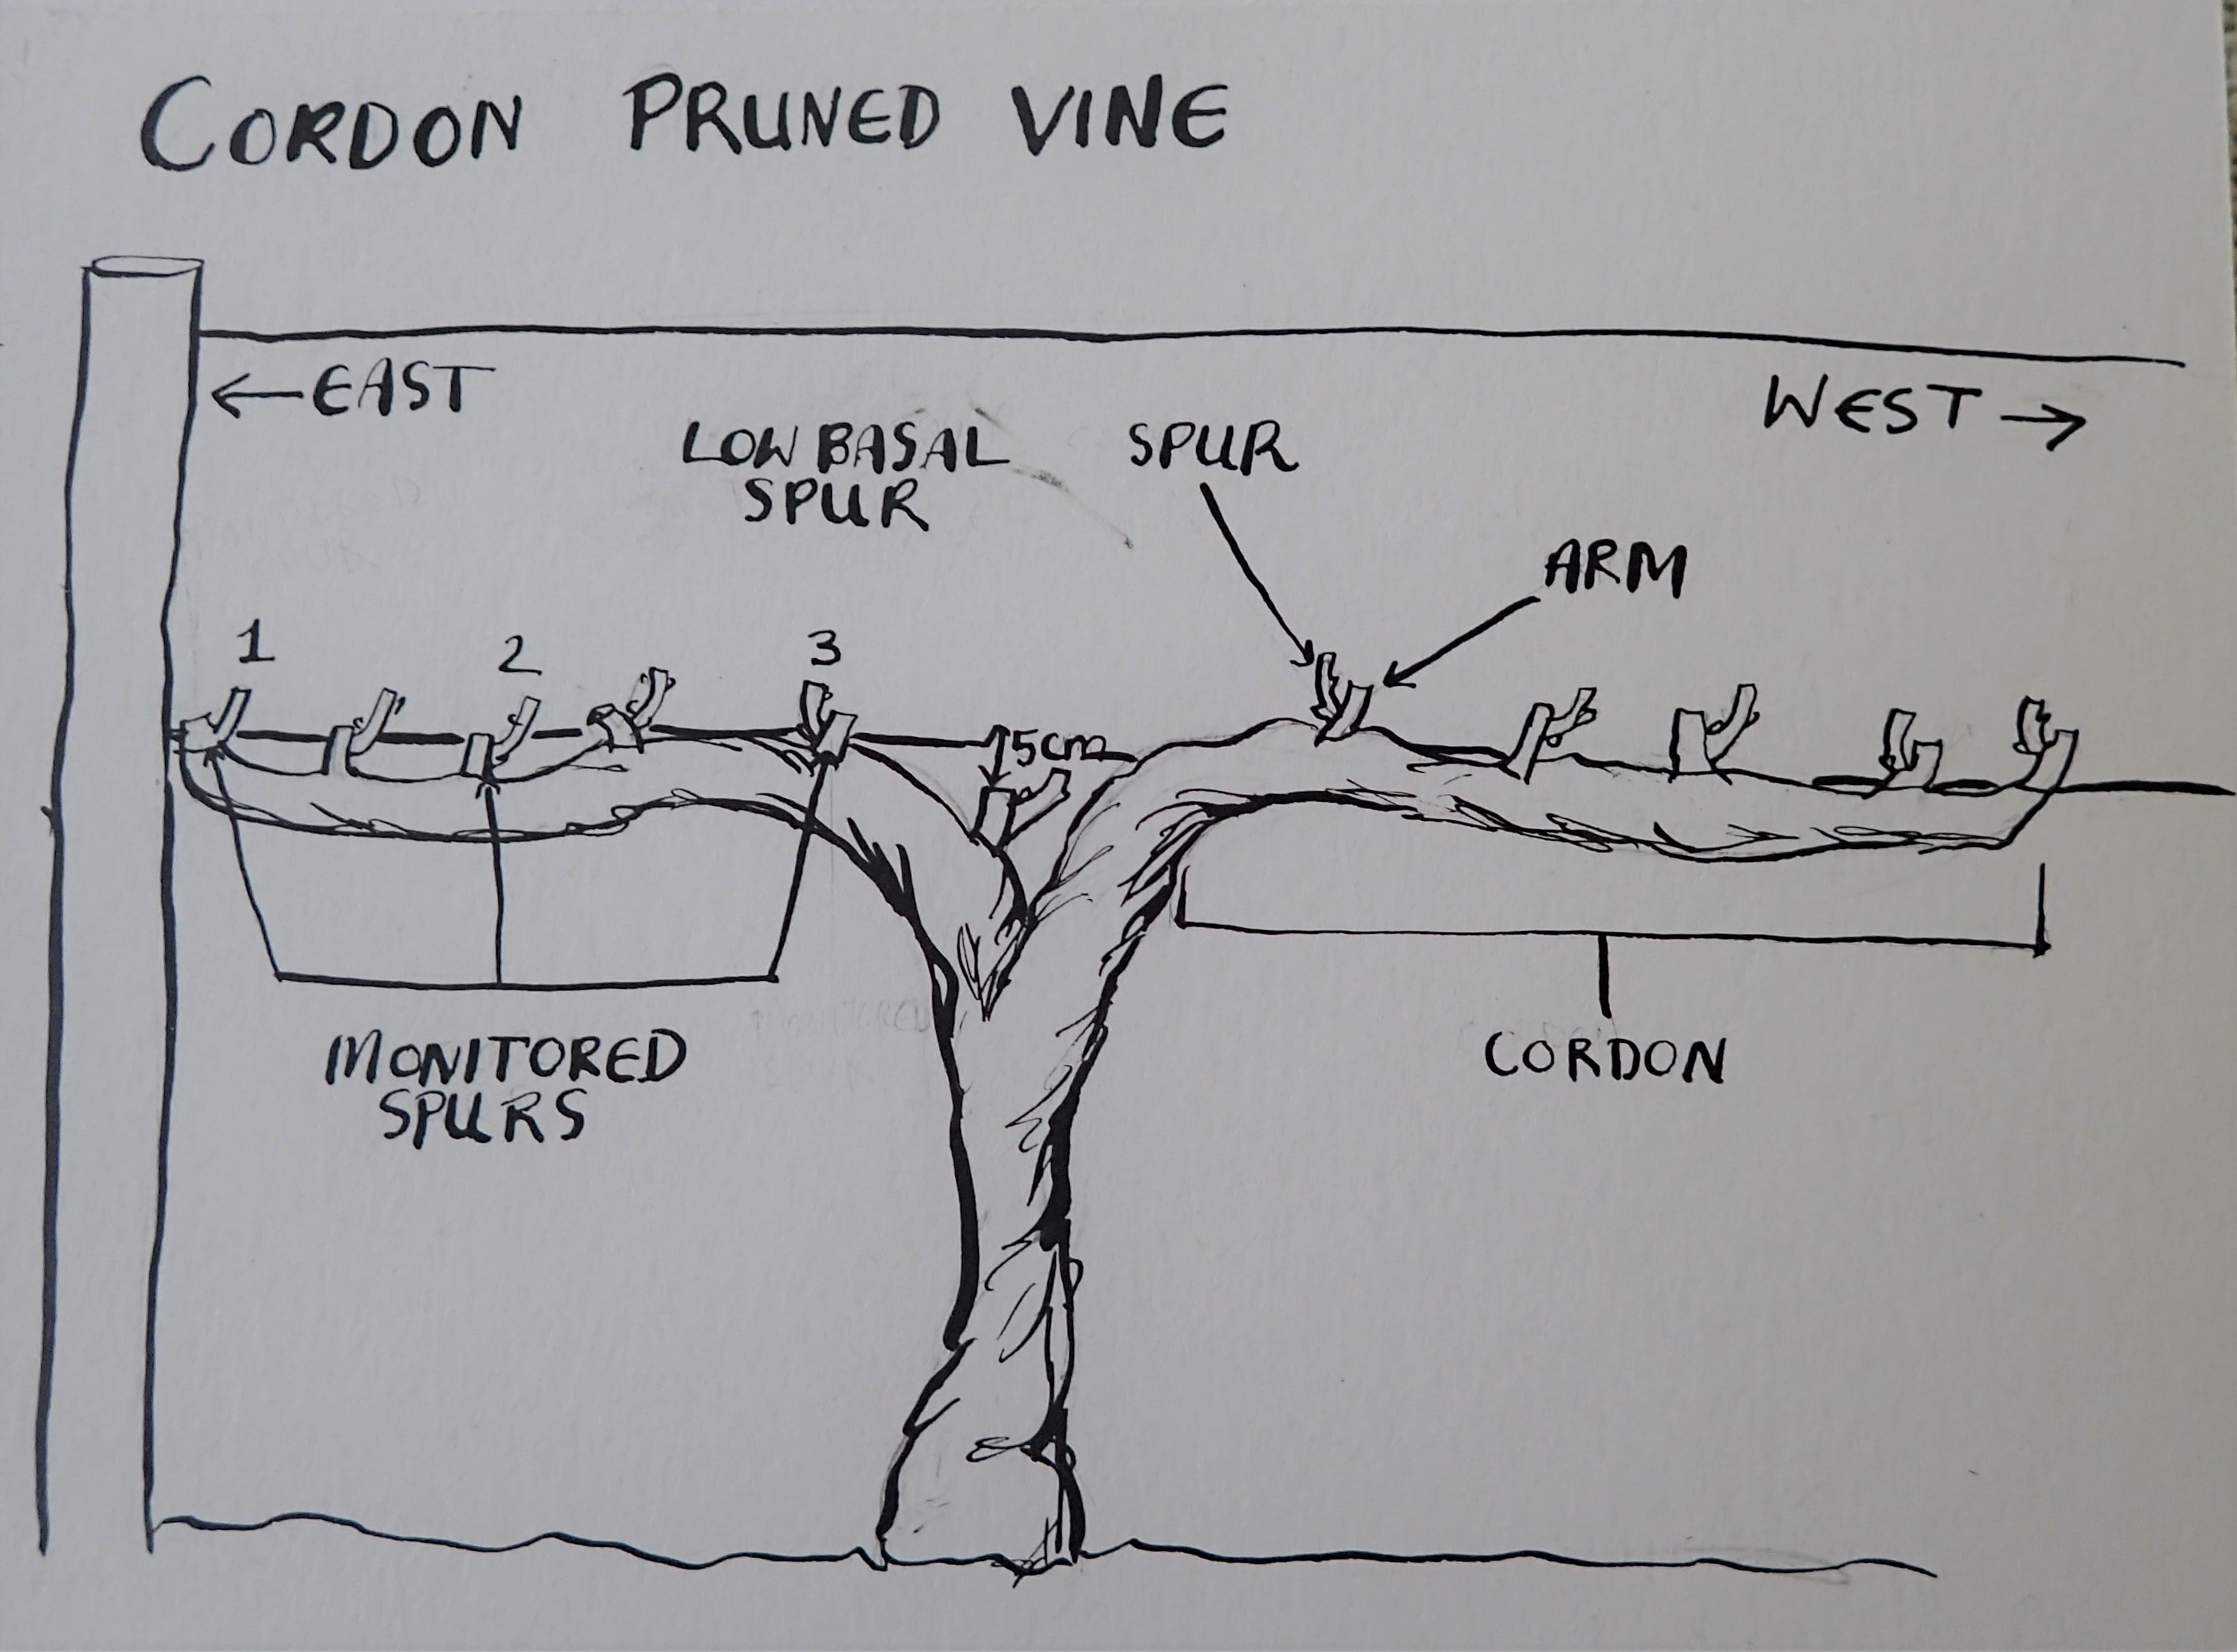
\includegraphics[width=\linewidth]{CordonPruned.jpg}
  \caption{A diagram of a cordon pruned vine, showing which spurs we would monitor and their numbering. Any spur that's base was more than 5cm below the wire the cordon was trained on was not sampled.}
  \label{fig:CordonPruned}
\end{figure}

\begin{figure}
  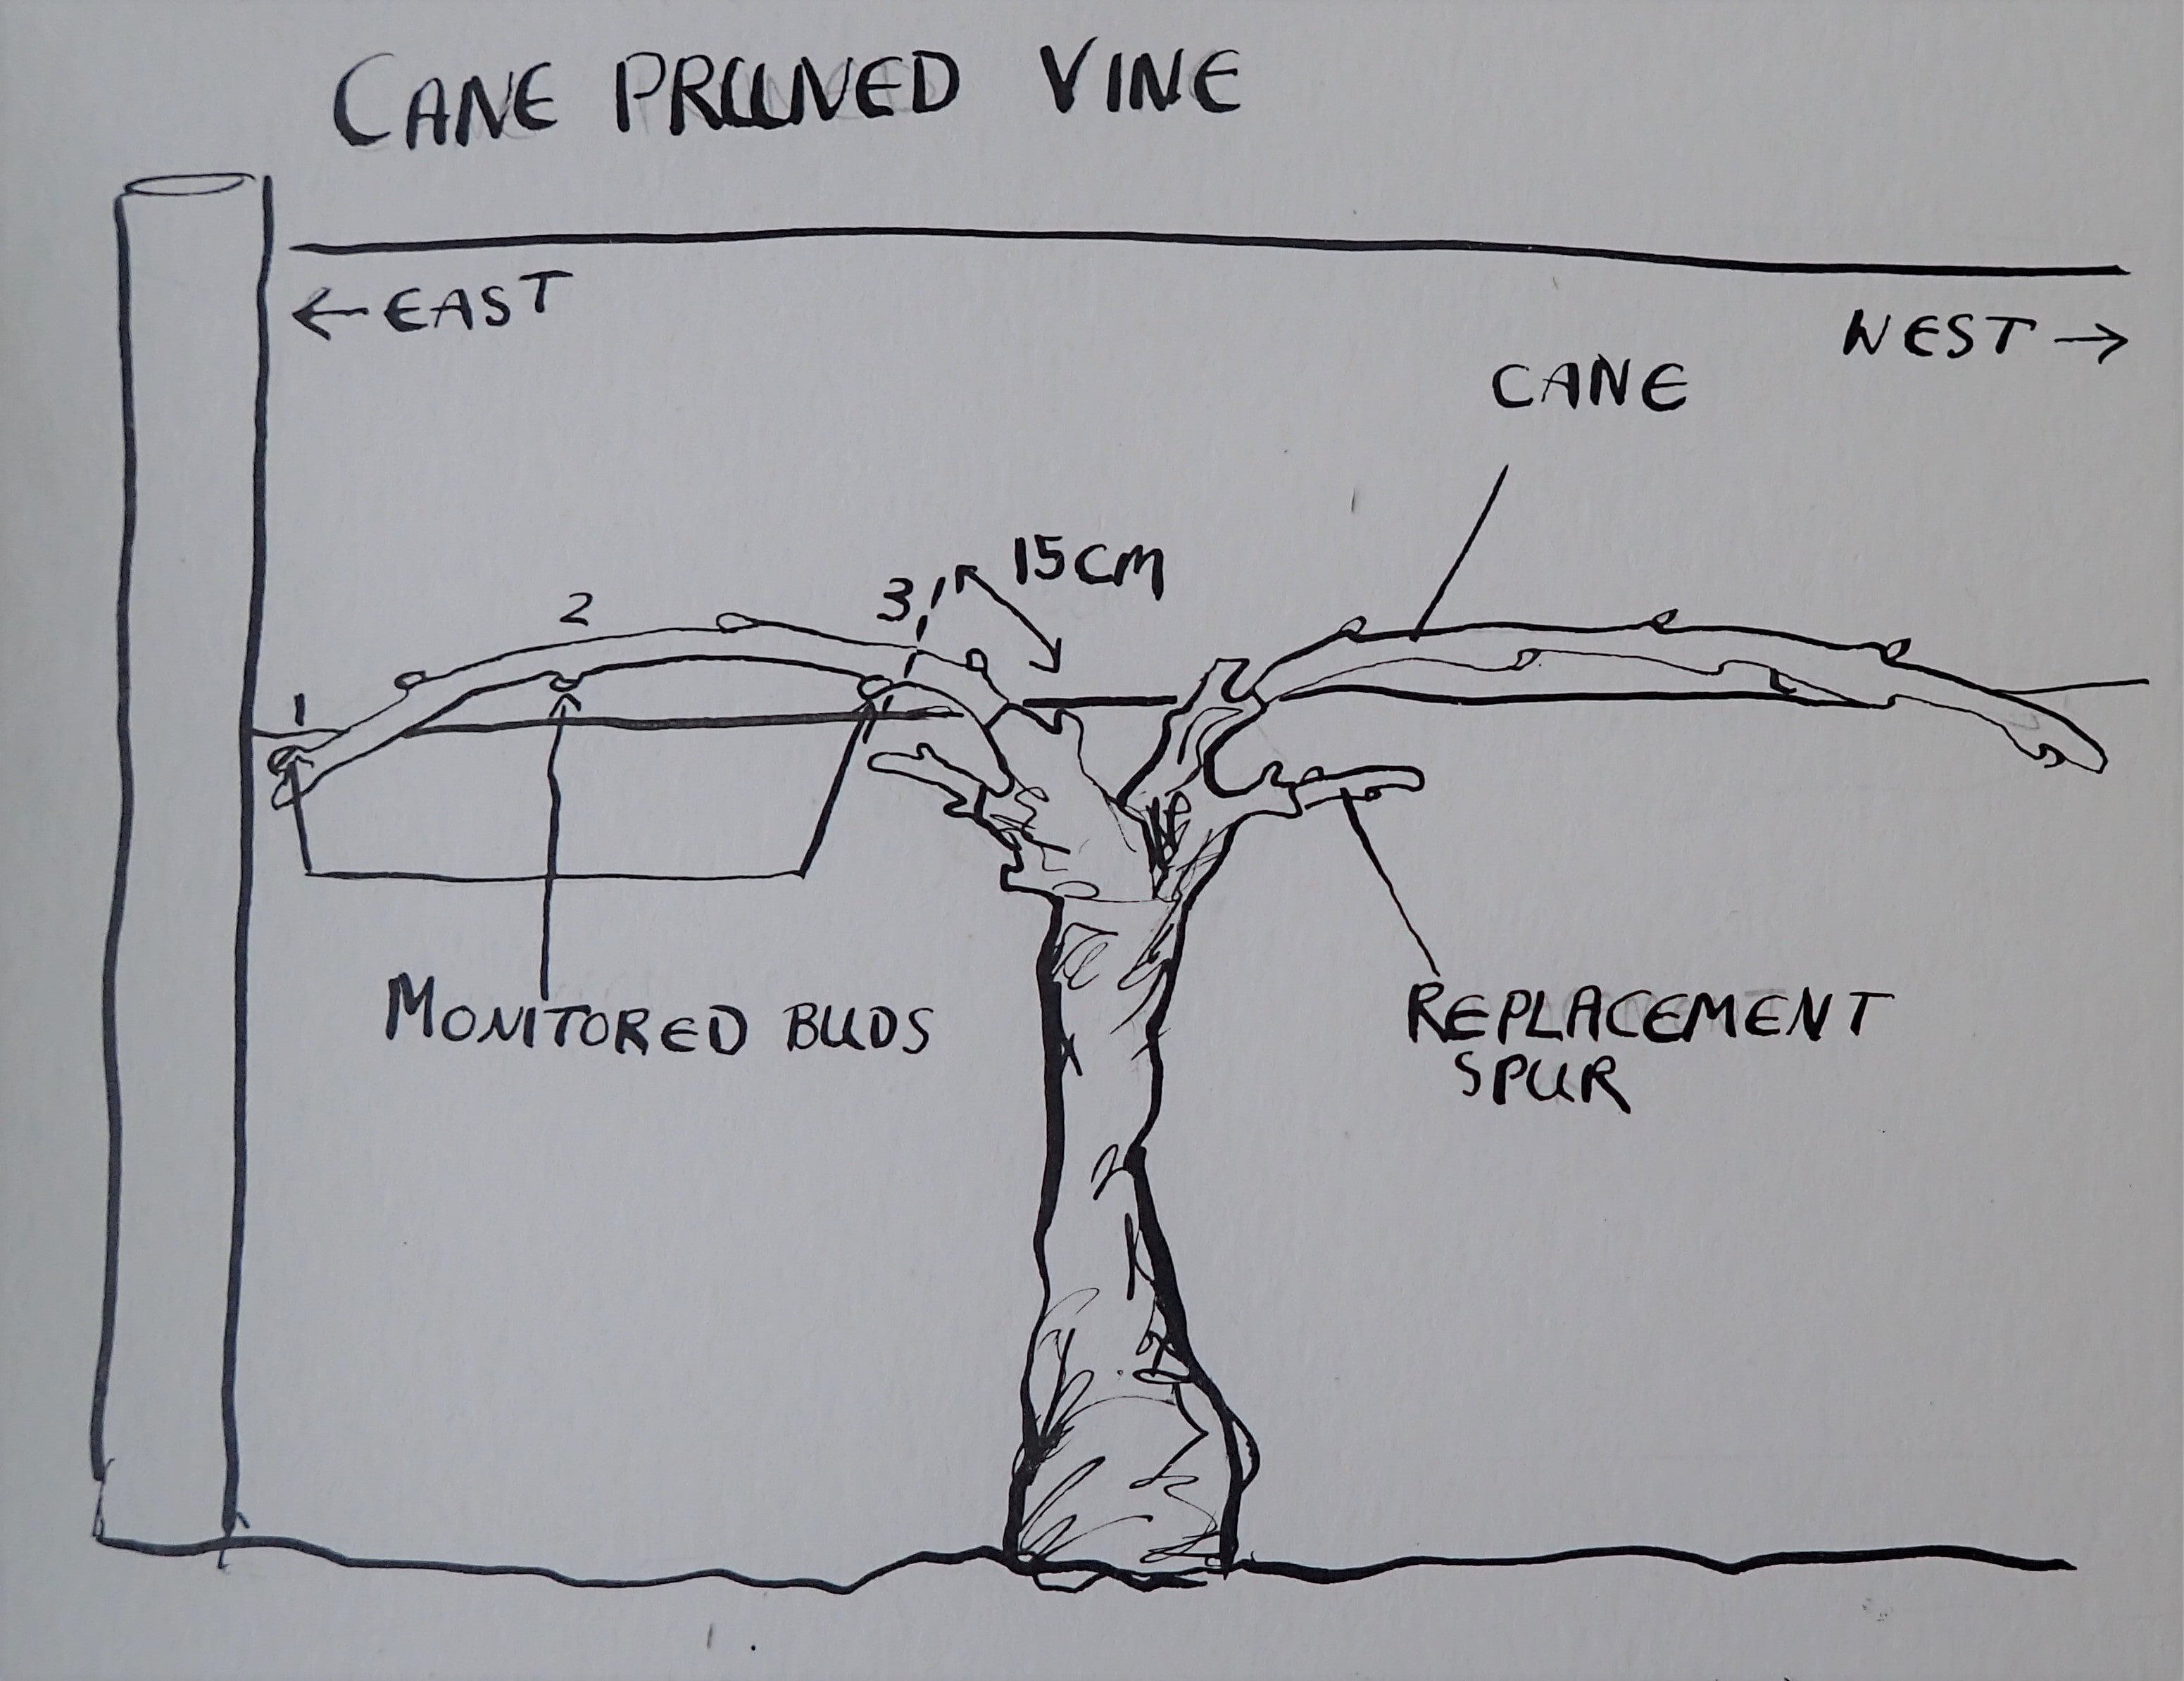
\includegraphics[width=\linewidth]{CanePruned.jpg}
  \caption{A diagram of a cane pruned vine, with the buds we would monitor and correct bud numbering. Note that we do not sample buds too close to the head of the vine.}
  \label{fig:CanePruned}
\end{figure}

\begin{figure}
  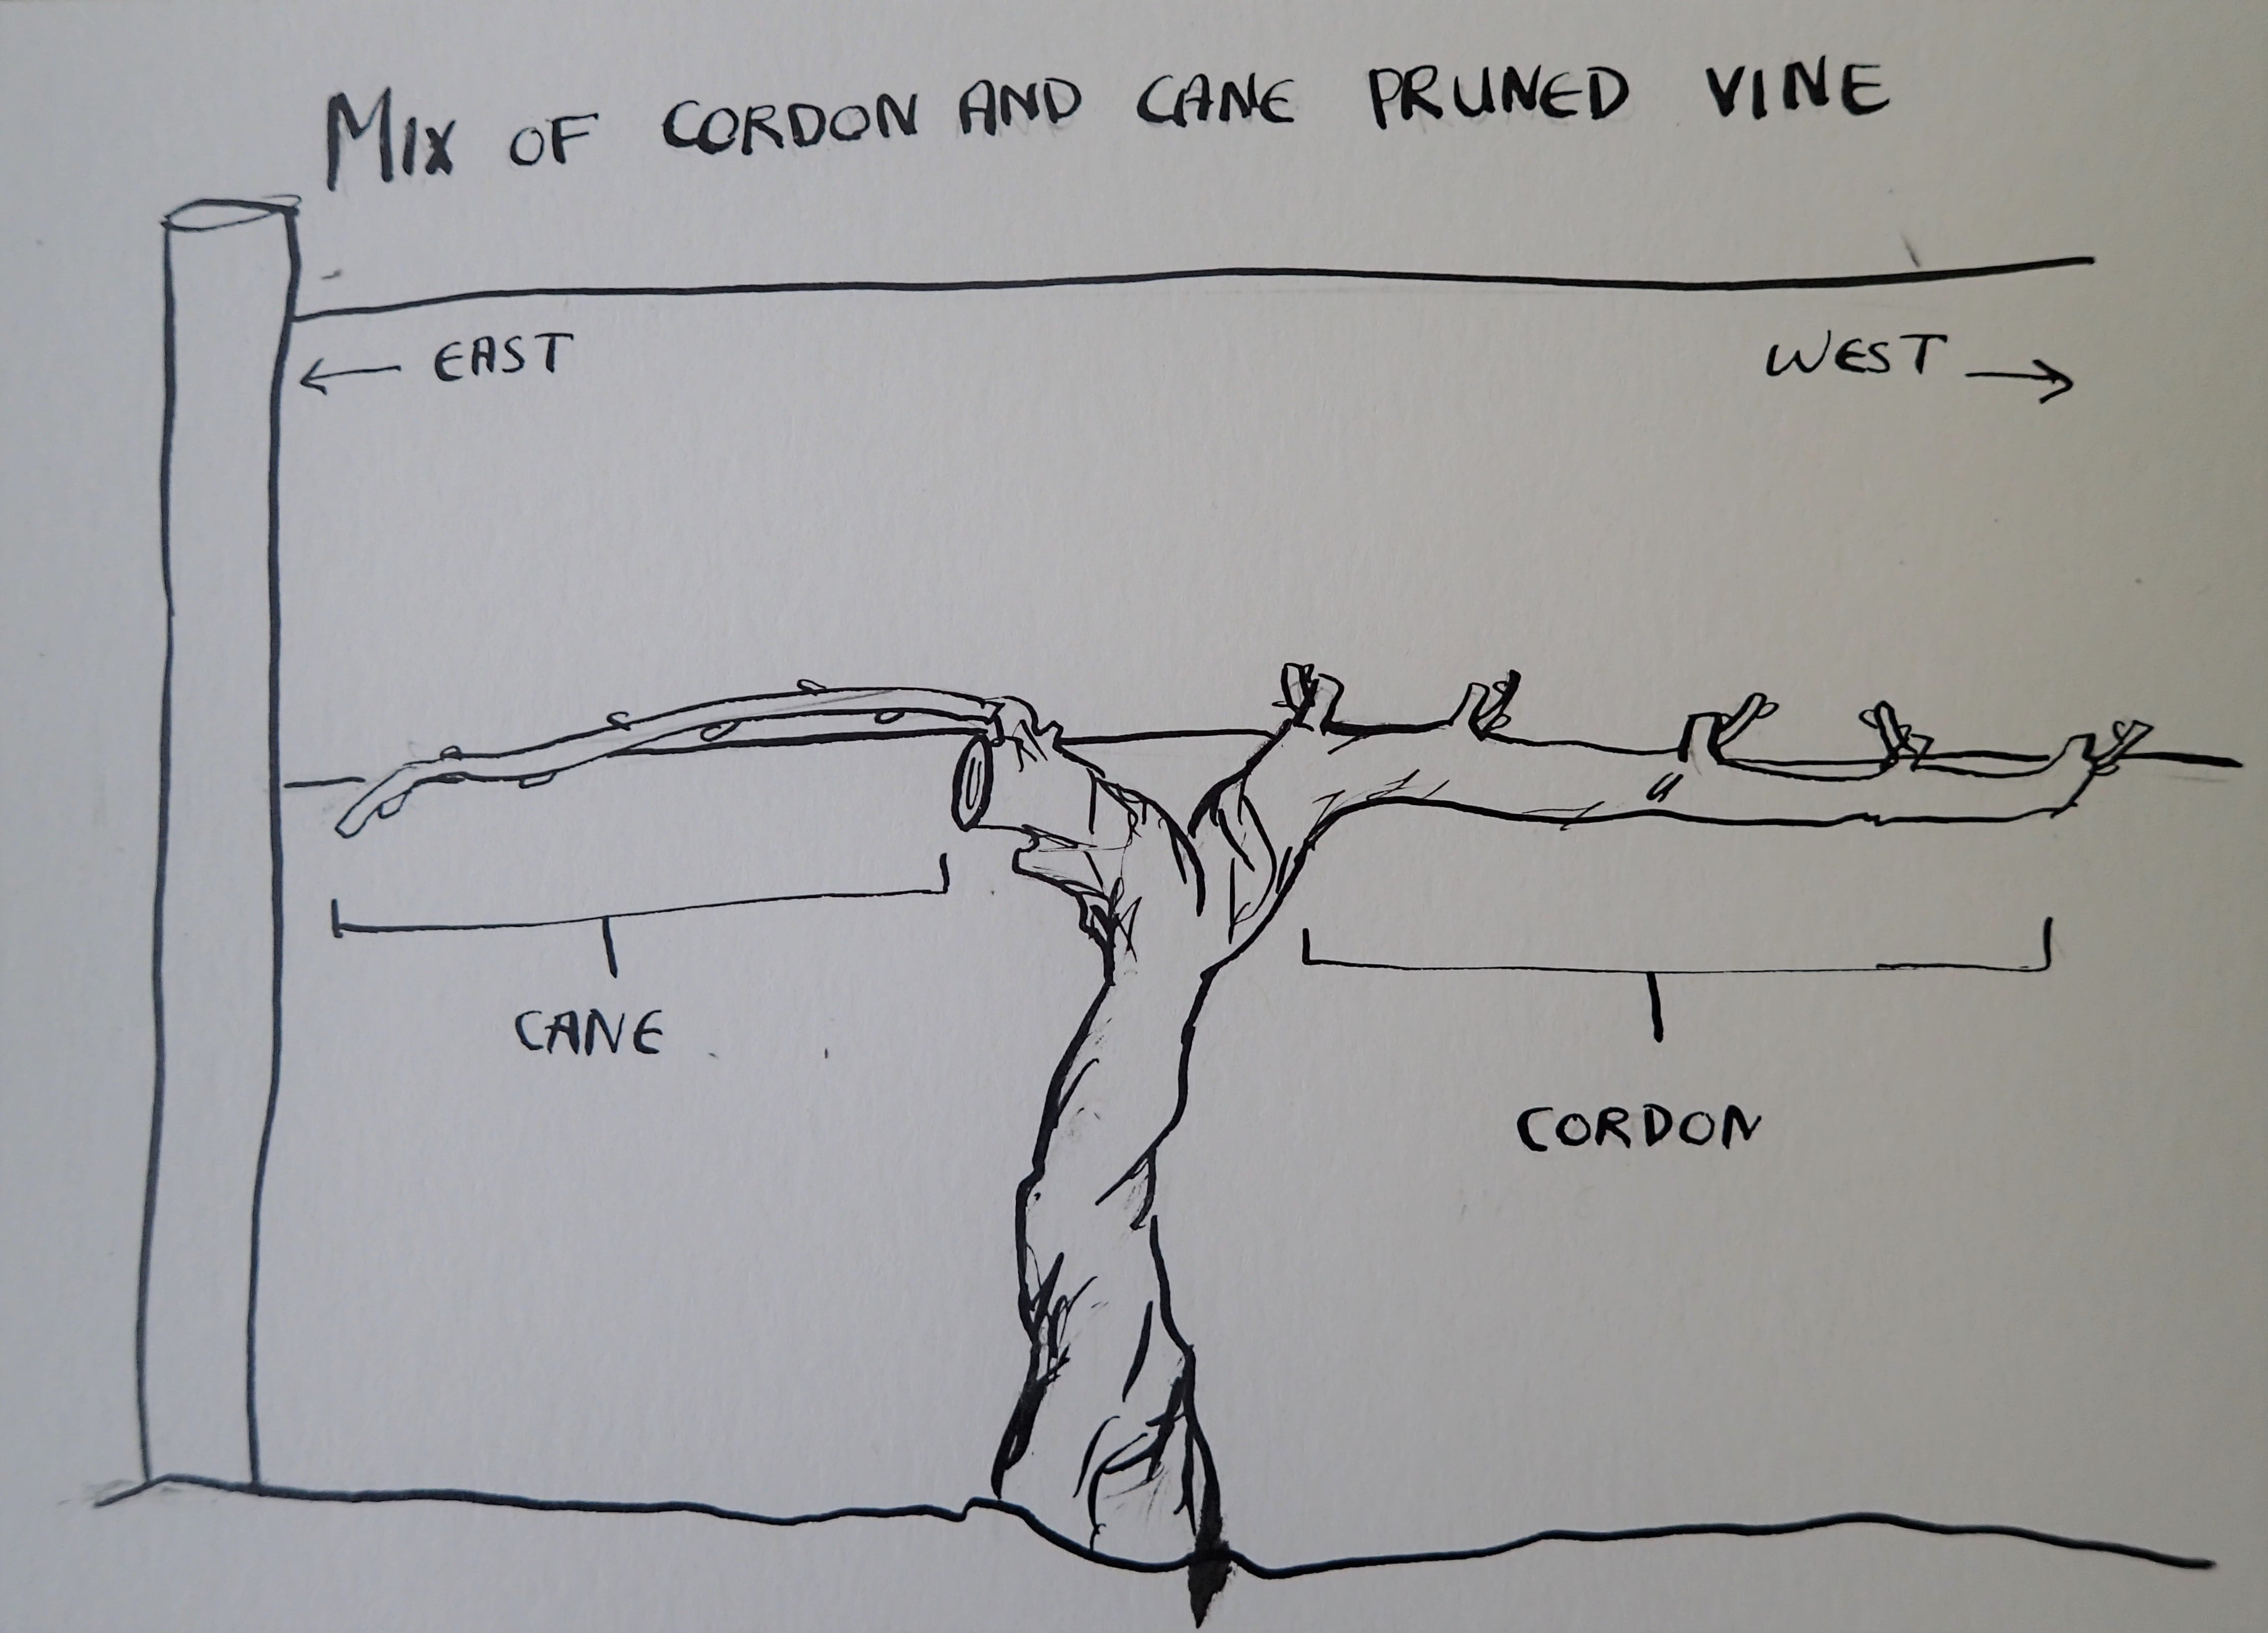
\includegraphics[width=\linewidth]{CaneCordonMix.jpg}
  \caption{When there is both a cordon and a cane, you we sample the cordon unless the cordon has less than three spurs.}
  \label{fig:CordonCane}
\end{figure}

\begin{figure}
  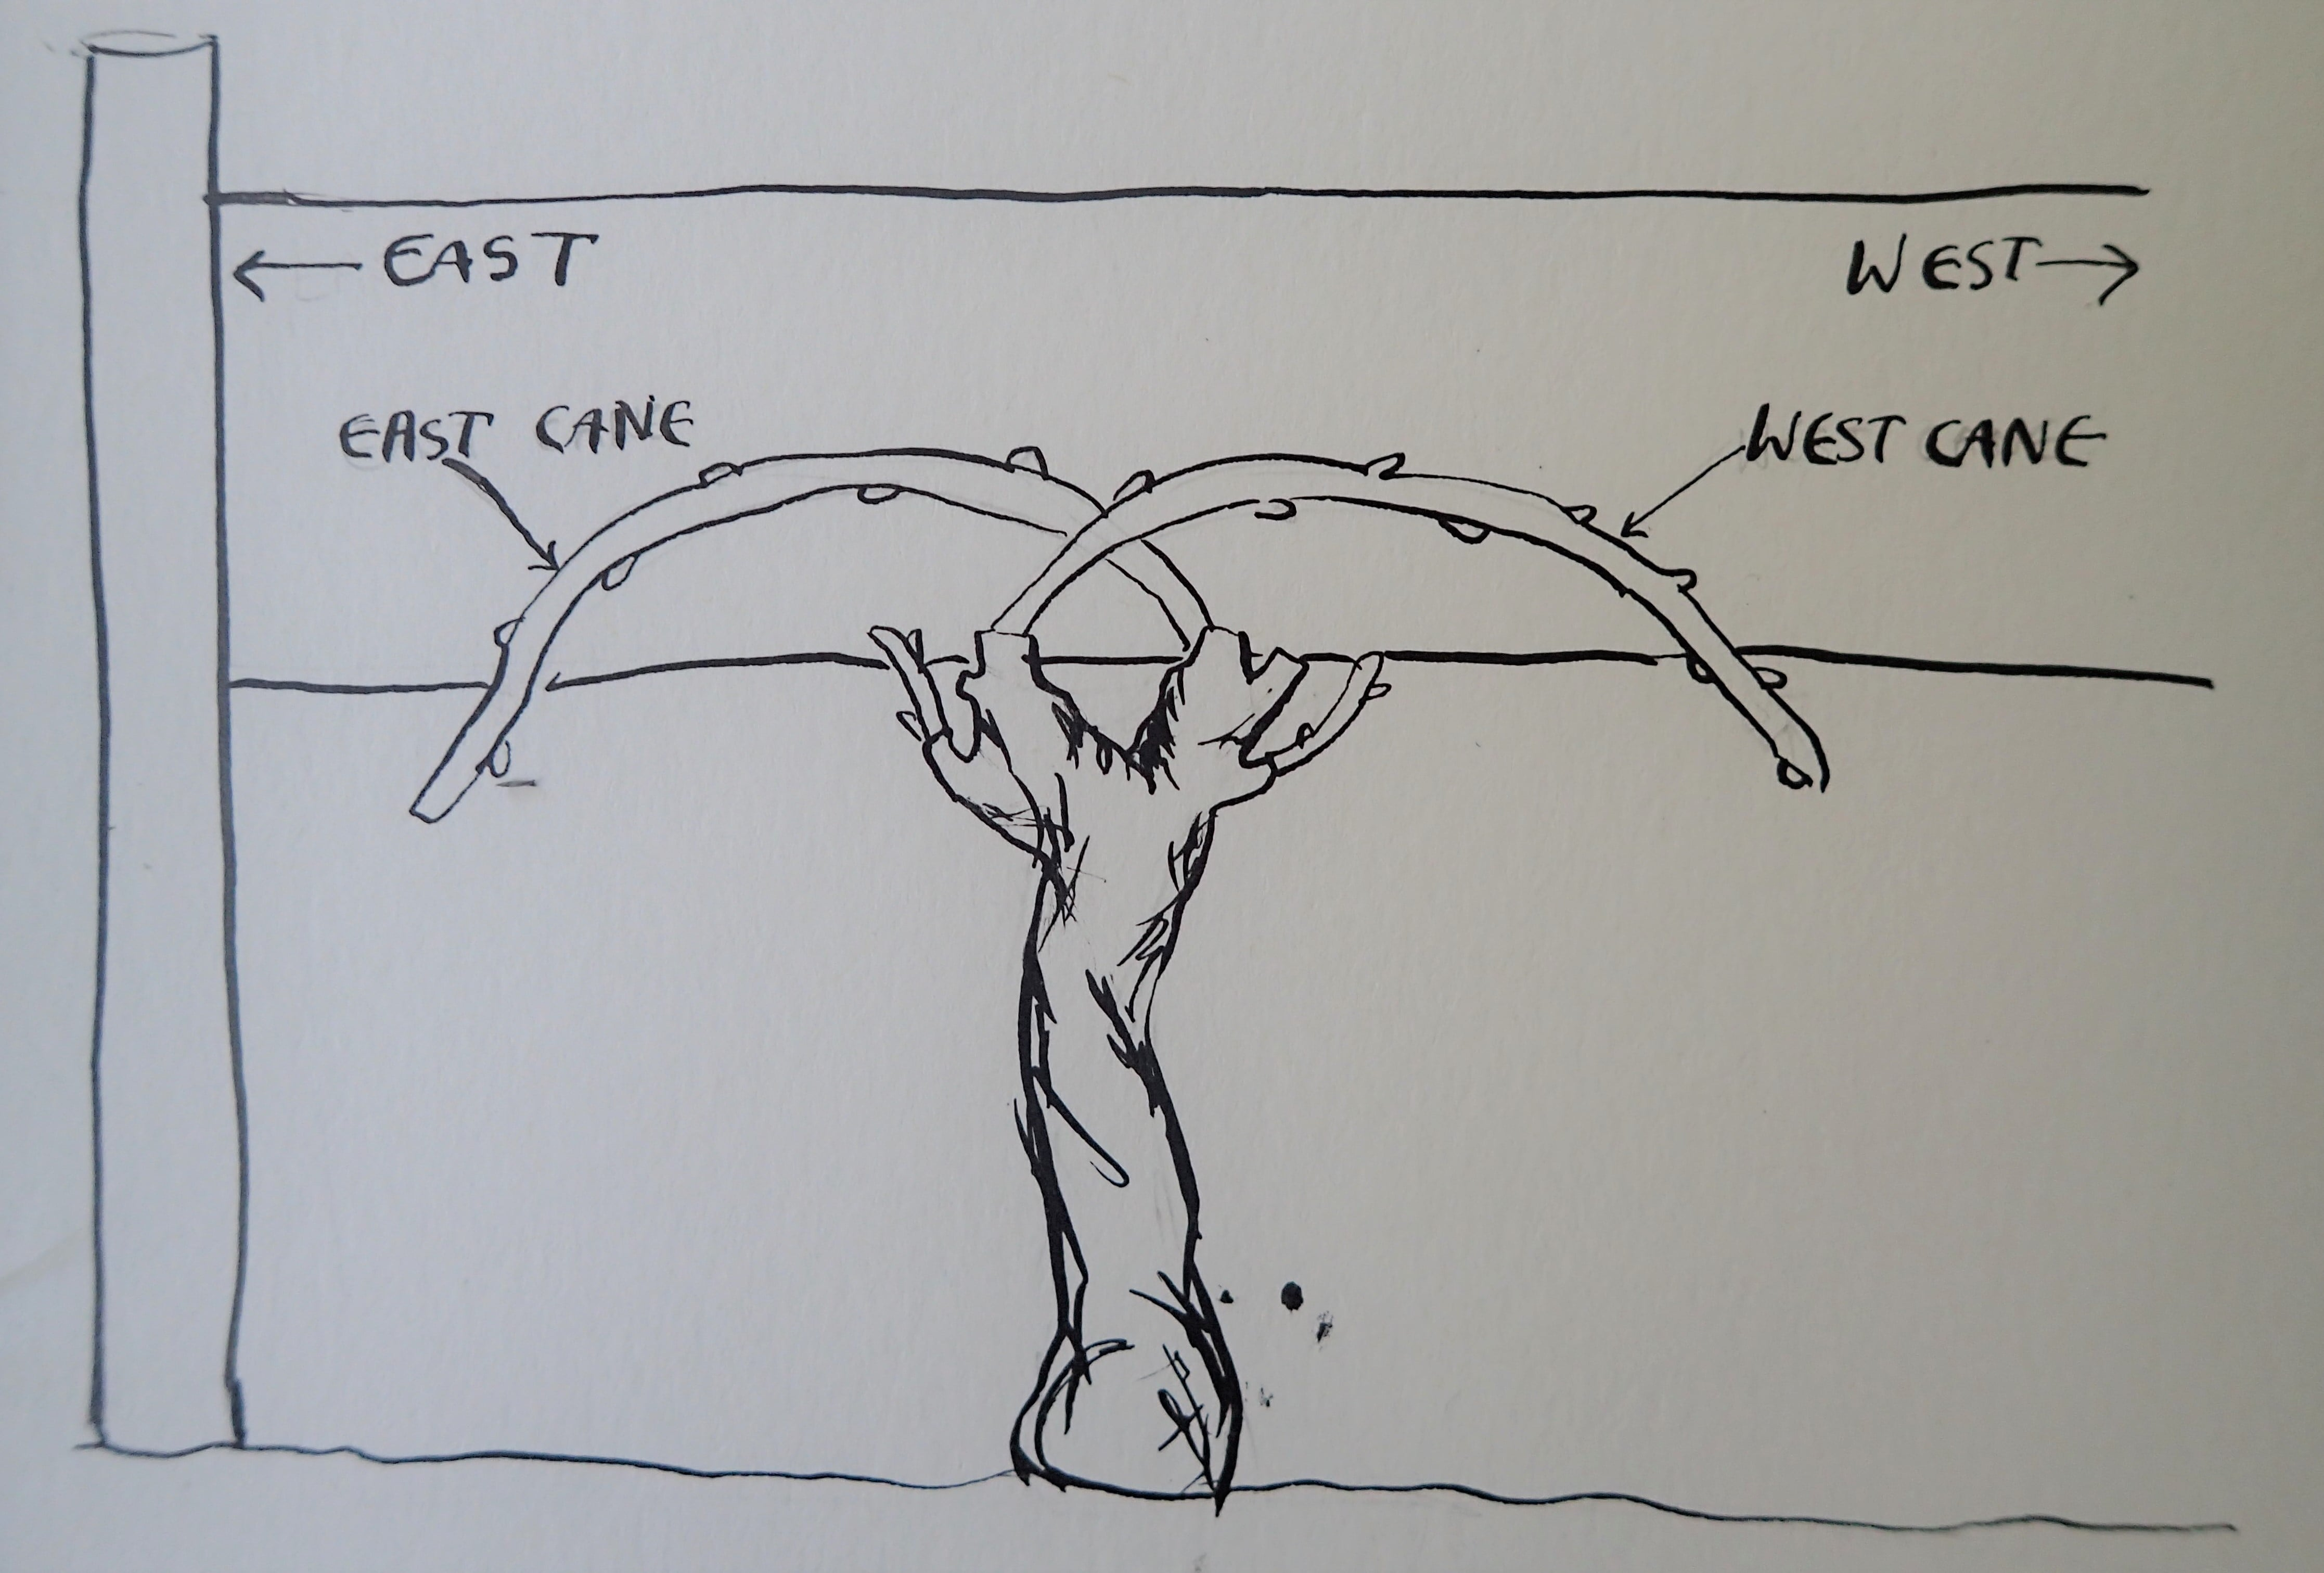
\includegraphics[width=\linewidth]{CaneCrossing.jpg}
  \caption{Sometimes the canes are crossed. If they do, we use the end of the cane to decide which side is east/west or north/south.}
  \label{fig:CaneCrossing}
\end{figure}

\begin{figure}
  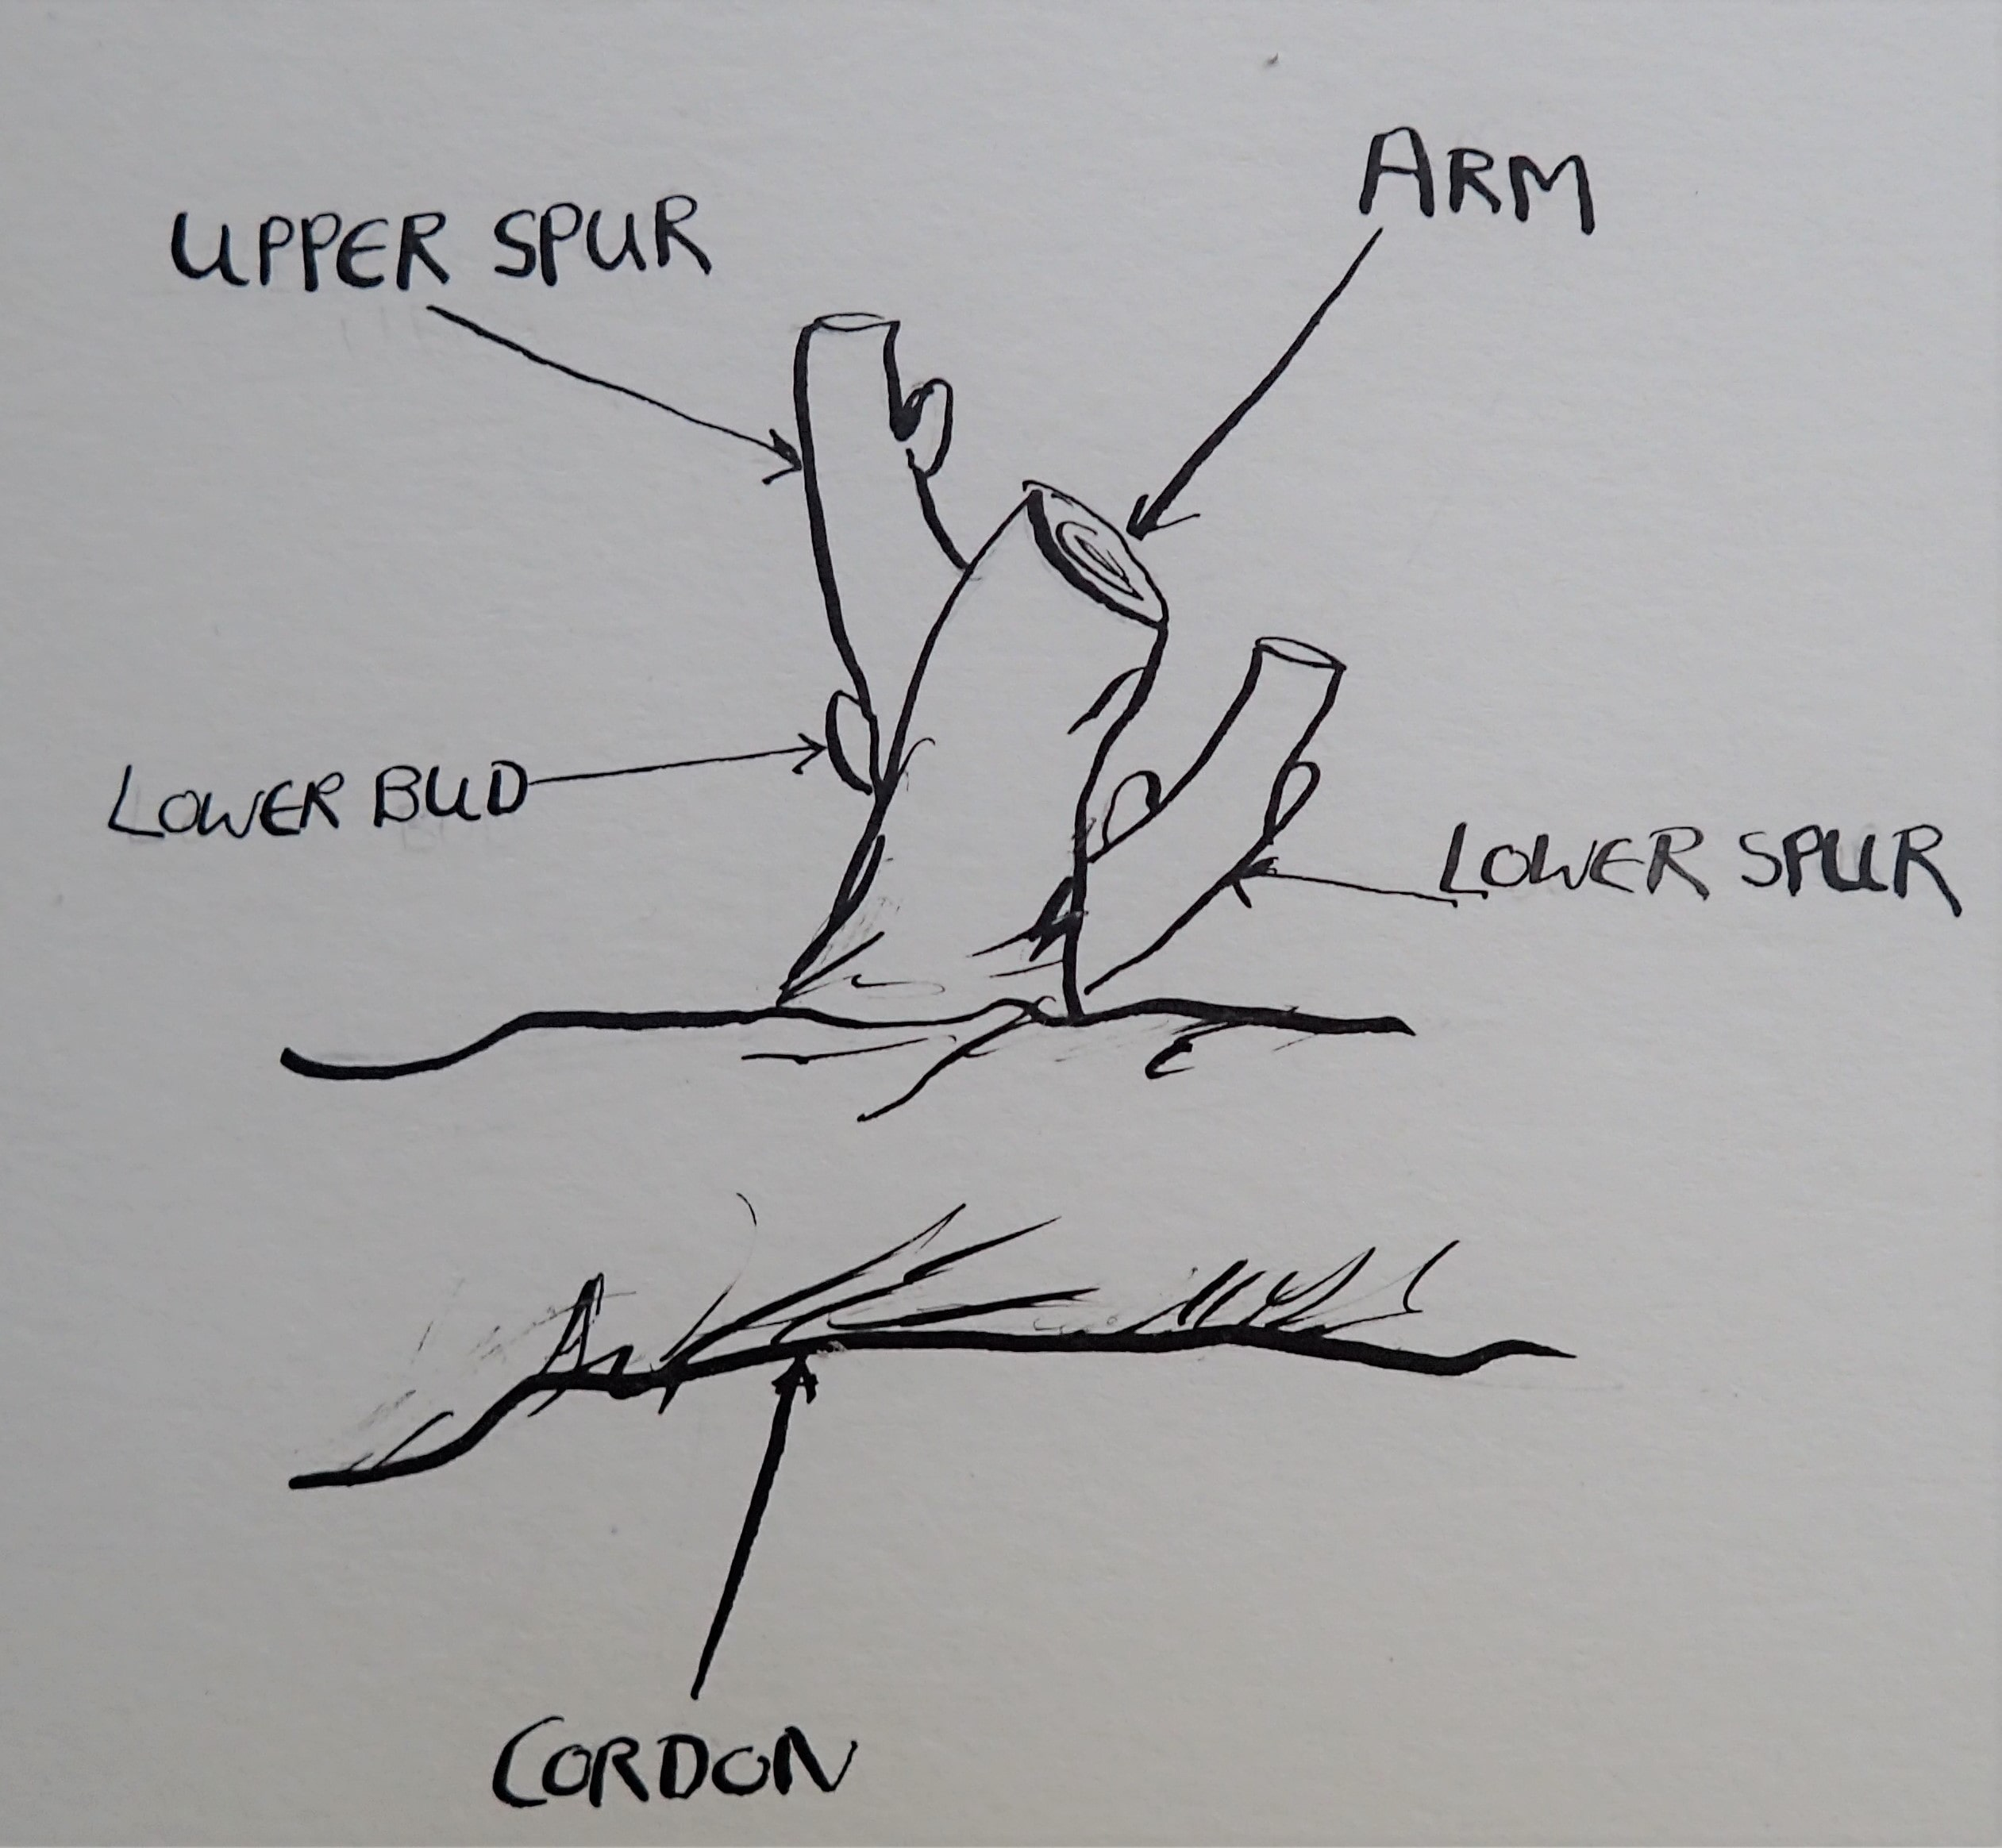
\includegraphics[width=\linewidth]{TwoSpurs.jpg}
  \caption{A diagram of an arm of a cordon that had two spurs on it. In this case we chose to focus on the lower bud of the higher of the two spurs for monitoring.}
  \label{fig:TwoSpurs}
\end{figure}

If plant was either cordon pruned (Figure \ref{fig:CordonPruned}) or cane pruned (Figure \ref{fig:CanePruned}, we flipped a coin to determine which side was flagged (heads = south or east, tails = north or west). If one side of the plant did not have enough buds, we chose the other side. When the cordons were clearly different ages, we chose to sample the larger/stronger cordon because it will be more representative of the plant. If a plant had a cane and a cordon (Figure \ref{fig:CordonCane}), we flagged the cordon unless it did not have at least three spurs, then the cane was flagged. Occasionally, a cane would be trained back to the trunk in a loop or had come loose from the wire. In these cases, we flagged the other cane. If the cane started on one side but was trained to cross over and end on the other side, we used the direction of the end of the cane. (Figure \ref{fig:CaneCrossing})


\subsubsection{Cordon Buds}

We flagged the spur (or arm if it was present) on the furthest from the trunk, a middle spur, and the first spur on the cordon with a base less than 5cm below the wire (Figure \ref{fig:CordonPruned}). Spurs 5 cm or more below the wire were considered basal. If there was an even number of spurs, a coin flip determined which middle spur was chosen. \\

If there was more than one spur on an arm (Figure \ref{fig:TwoSpurs}) then we focused on the higher spur. We monitored the lowest bud on this spur. 

\subsubsection{Cane Buds}

We flagged the bud furthest from the trunk, the middle bud, and the first but that was farther than 15 cm from the trunk (Figure \ref{fig:CanePruned}). If there was an even number of middle buds, a coin flip determined which bud was chosen. \\

If there were two buds in the same place in a position that was flagged, we chose to monitor the bud that was more upright. If both buds were equally upright facing, we monitored the one in a southerly or easterly direction. 

\subsection{Numbering Buds}
For the first set of data collection, Mira and Faith numbered the buds on each cordon or cane from 1 to 3 in ascending order from either the south or the east. This caused confusion in the field so we decided to change the numbering protocol. {\bf For data entry: the numbering for all east and south cordons/canes should be reversed, the numbering for north and west cordons/canes is fine (buds are numbered 1 to 3 from trunk)} \\

{\bf For the Dark Horse monitoring protocol and future years, use the following protocol}:
Number buds 1 to 3 with bud 1 being the bud closest to the trunk (see Figures \ref{fig:CordonPruned} \& \ref{fig:CanePruned}). 

\subsection{Choosing Clusters}
From each bud selected for monitoring during budburst, a cane will arise bearing one or more clusters of grapes. For the remaining pheno stages (bloom, veraison, Brix), we want to select a specific cluster for monitoring rather than a cane. Select the basal cluster (the lower one, originating closest to the ground) on the chosen cane (which will arise from the lowest bud position on the flagged arm, see Choosing Buds section) (Figure \ref{fig:TwoBunches}). This will generally be the strongest cluster; especially in warm climates, there may be a big developmental difference between upper and lower clusters on the same shoot (Figure \ref{fig:Bunches}). \\

This cluster will first be visible during the first pass for bloom. Note the lowest cluster on the first pass and make sure the same cluster will be monitored throughout the rest of the season. If you feel it will be difficult to keep track of the monitored cluster you can loosely ({\bf loosely!}) flag it. Do not flag tightly before this as it can prevent the growing tissue from maturing regularly. If a flagged cluster dies, disappears or somehow becomes no longer suitable for monitoring: Reflag nearest cluster and note in datasheet. In no case should you select, flag, or sample from a cluster that is more than 3-4 nodes along the cane (such a 'second crop' cluster will not be representative). \\

Once the green vines become woody (this is often after flower set or post-scatter, that is when you can shake the cluster and a few berries fall off) you can flag the cluster normally. You will take all remaining phenological samples from this cluster. It is important to flag the cluster to ensure repeatability in subsequent samplings by the same observer across different days (or by different observers). If possible, use the flag from the bud. It may seem obvious at this early stage, but the selected cluster can get a lot more confusing with subsequent growth throughout the season.

\begin{figure}
  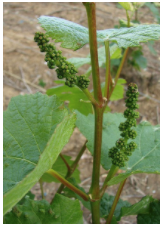
\includegraphics[scale = .75]{TwoBunch.png}
  \caption{The basal cluster (right) should be flagged rather than the second cluster (left) }
  \label{fig:TwoBunches}
\end{figure}

\begin{figure}
  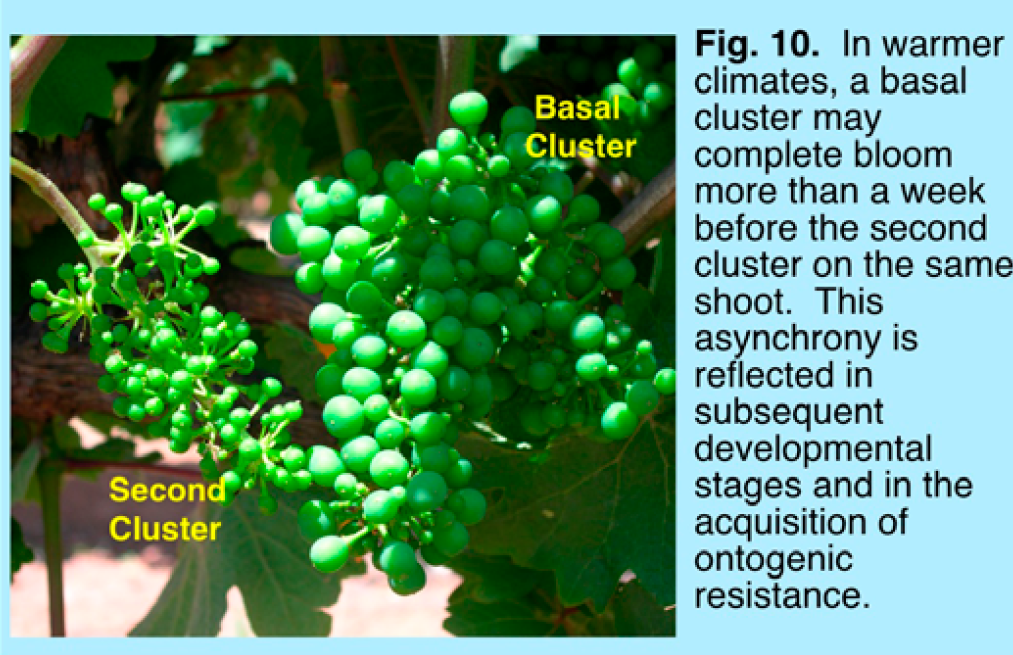
\includegraphics[scale = .25]{Gadoruy2012Bunches.png}
  \caption{(labeled Figure10 in image). Source: Gadoury et al. 2012, \url{http://grapesandwine.cals.cornell.edu/cals/grapesandwine/appellation-cornell/issue-11/loader.cfm?csModule=security/getfile&PageID=1074171}}
  \label{fig:Bunches}
\end{figure}

\begin{figure}
  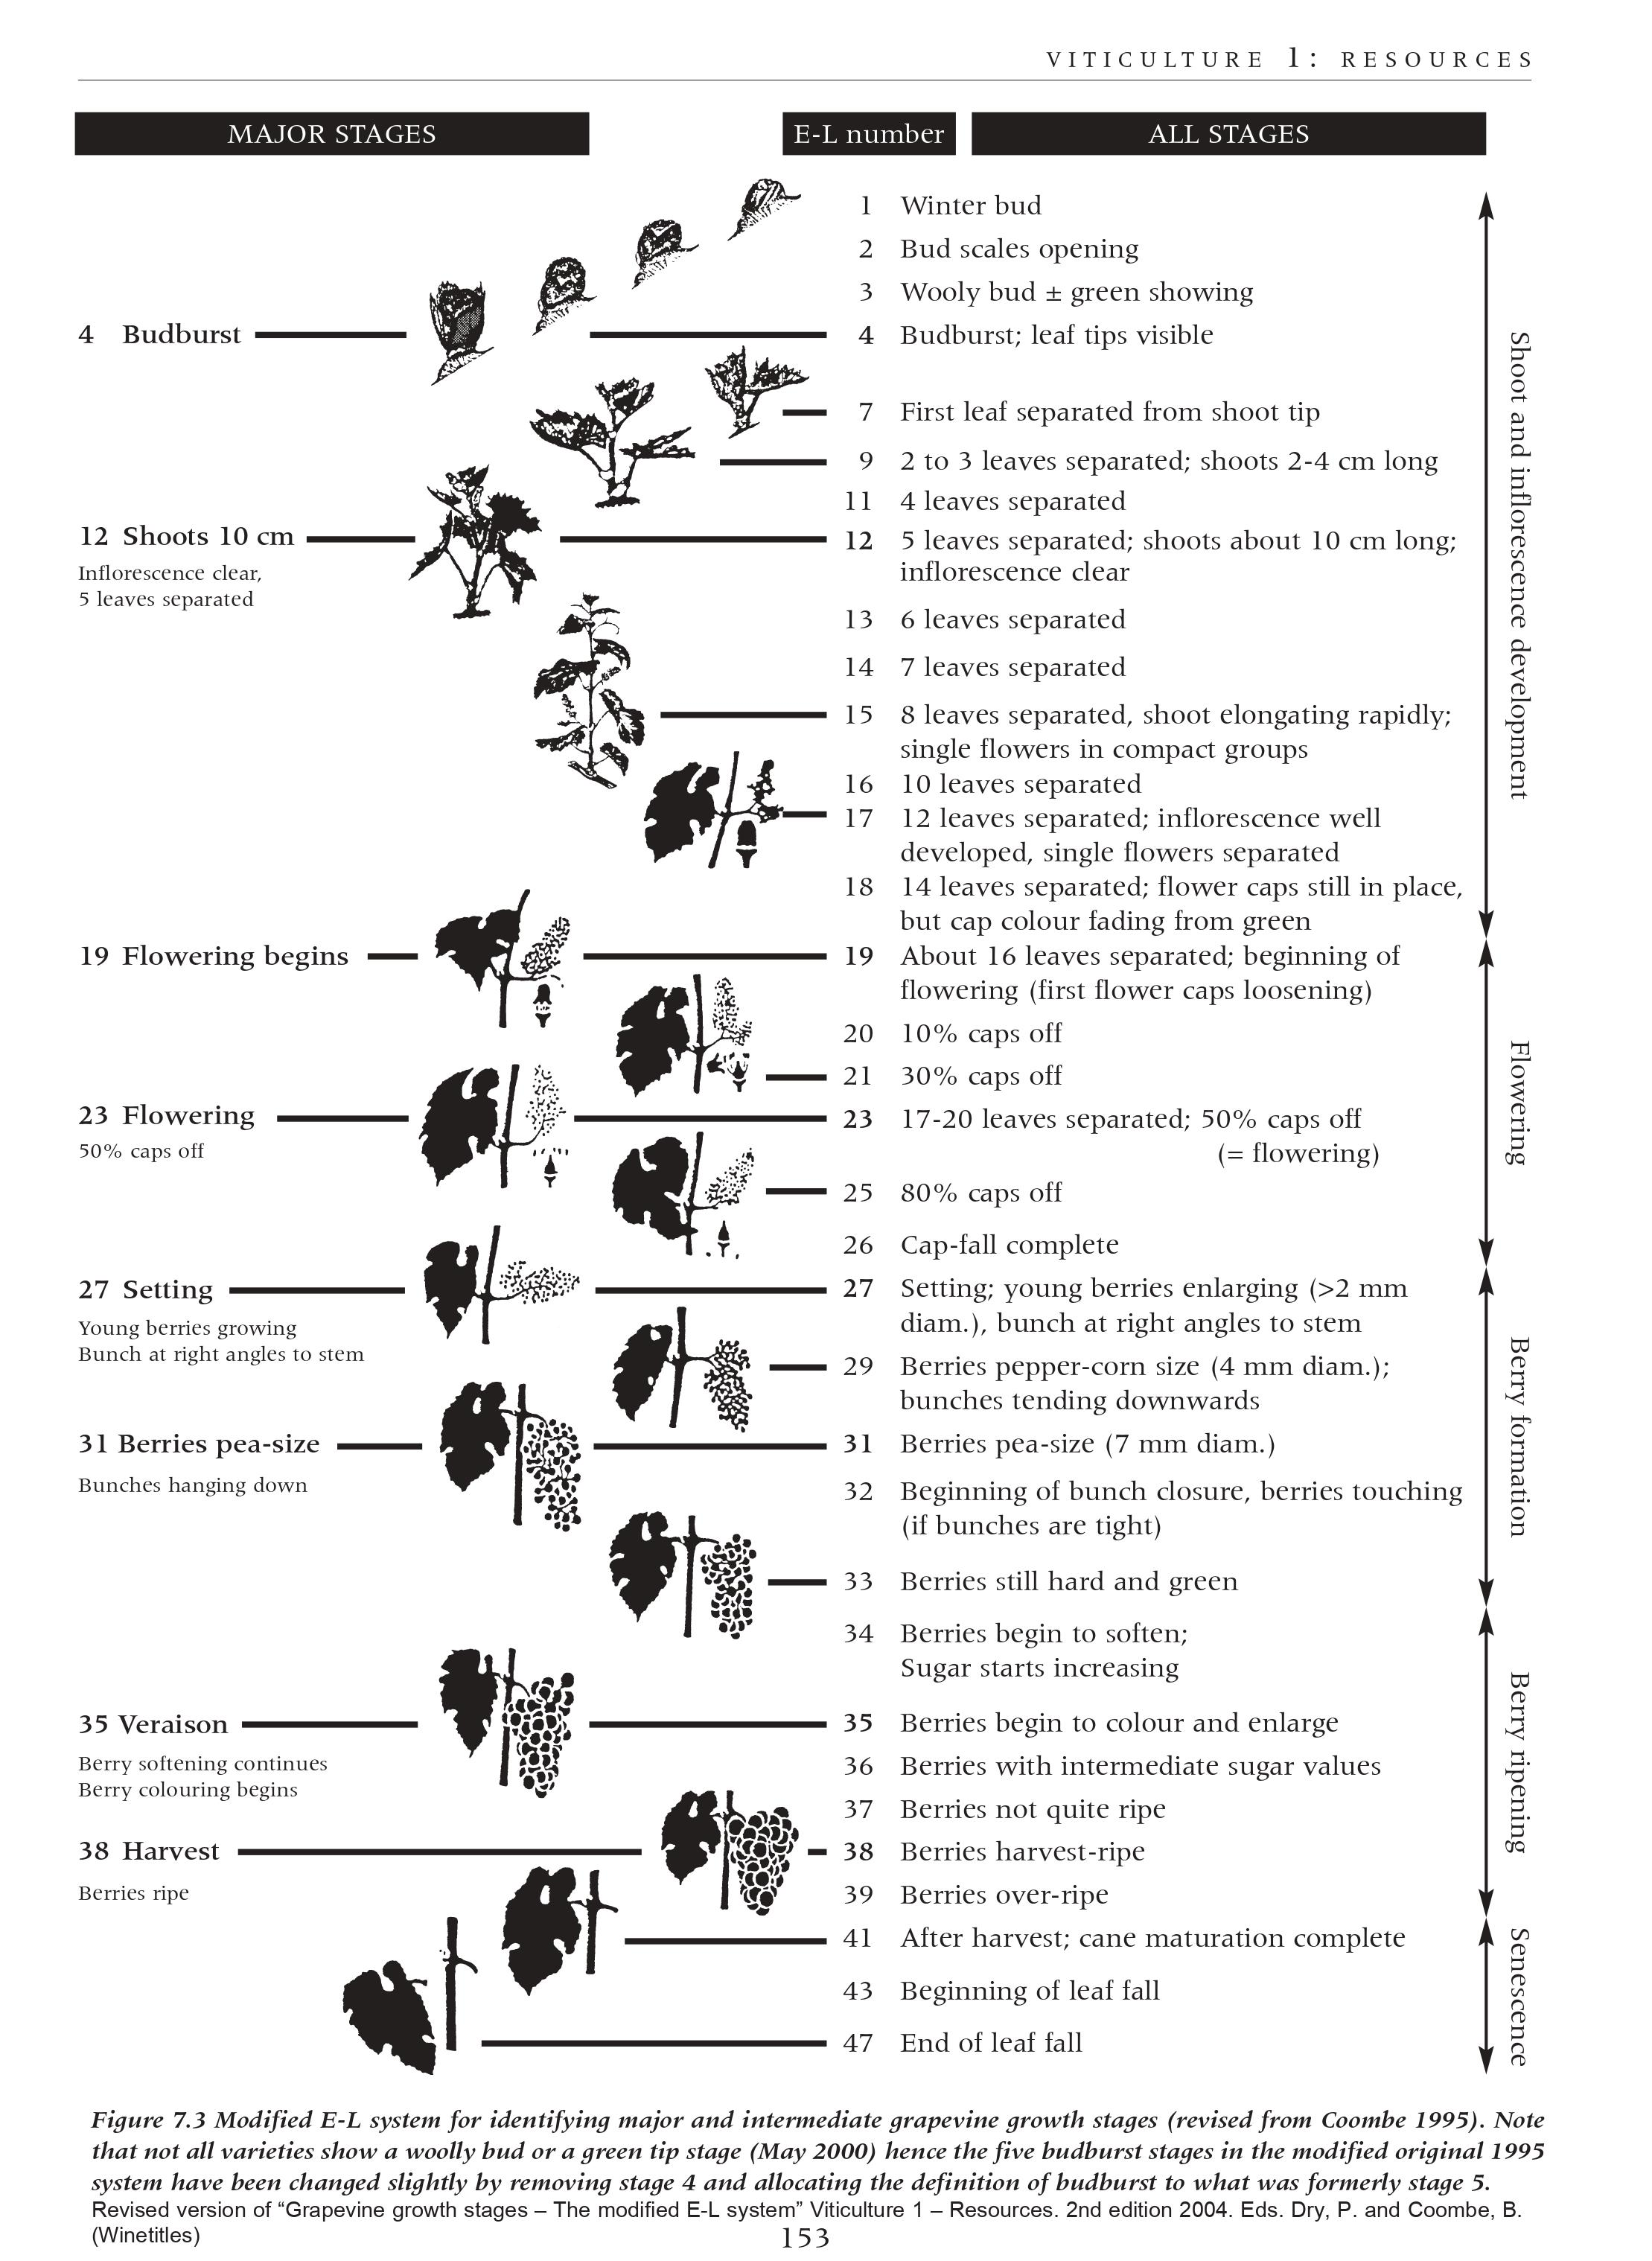
\includegraphics[width=\linewidth]{ELScale.jpg}
  \caption{ Modified Eichorn-Lorenz (EL) scale that our lab uses for monitoring phenology until flowering. There are different versions of Eichorn-Lorenz so please follow this one! }
  \label{fig:ELScale}
\end{figure}

\section{Monitoring}
Our goal is to have standardized observations of phenological stages for analysis. There are four main widely observed stages for winegrapes: (1) budburst, (2) flowering, (3) veraison, and (4) ripening and harvest. For the first stage, budburst, we will use the stage numbers from the Modified Eichorn-Lorenz system (see Figure \ref{fig:ELScale}). For flowering and veraison, we will estimate the percent occurrence of the stage (proportion of berries on a selected cluster have gone through the stage of flowering or color change/softening, respectively). We will measure ripening quantitatively, using a refractometer to measure Brix.

\subsection{Sampling Frequency and Timing}

\begin{enumerate}
\item We monitor four phenological stages: 
	\begin{smitemize}
	\item Budburst (approx. mid-April - mid-May): Until EL stage 12, record the EL stage of buds on three spurs. Once EL stage is at 12 you can stop recording until flowering starts (note that you may need to record higher than stage 12 at times in order to record whatever stage you see after 11, even if it is 13 or such if you have not yet recorded stage 12, more on this in Monitoring Instructions).
	\item Bloom (approx. June 1-30)
	\item Veraison (approx. Aug 1-30)
	\item Ripening (Brix - approx Aug 15-Sept 30)
	\end{smitemize}
\item We estimate that observing pheno stages for each vine (budburst, bloom, and veraison) will take approximately 90s per vine. 
\item Once at least 5\% of the phenological stage (i.e., 5\% bloom) is seen, go out to the field until stage is complete for all varieties being monitored. 
\item During peak sampling, we will aim for techs to make pheno observations every 3 days (2x/week) \emph{if possible}.  
\item Following the end of one pheno stage, techs will do a weekly vineyard walk-through starting 2-3 weeks before the anticipated beginning of the next stage, to make sure to catch early varieties entering the next stage. {\bf Let us know how this goes!} This is the first time the lab has worked in such a large climate gradient so we are unsure how much time there will be in the end between events (i.e., will there a period when no plants are undergoing flowering or veraison or will veraison start for early varieties in the south when flowering is still happening in the north?).
\end{enumerate}

\subsection{Fieldwork Prep}
Be sure to coordinate with vineyards before you visit to make sure you can access the vines. Generally the main issue is avoiding vines after spraying.\\

Field work materials:
\begin{smitemize}
\item Vineyard map
\item Sampling protocol
\item Description of grapevine phenological stages (see Figure \ref{fig:ELScale}, Modified Eichorn Lorennz system)
\item Field tablet for recording data
\item Pen/paper and data entry sheets as backup if tablet fails (print-outs of \verb|.xls| files)
\item Field notebook
\item Sharpie pens
\item Camera to record each stage for reference
\item Paper tags with attached string (like larger versions of yardsale pricetags) to help with labeling plants for photos 
\item Flagging tape for marking selected arms and clusters.
\item During ripening (August-September): Ziploc bags for berry collection.
\item Nice to have: paper towels \& handy wipes for cleanup (especially during Brix)
\item Hand sanitizer for use when touching any communal equipment, for example gates or portable washrooms.
\end{smitemize}

\subsection{Monitoring Instructions}
For each vine:
\begin{enumerate}
\item Stand facing the vine. Double-check Plant ID (labeled on one of the flags), block, and row number before recording in correct place on data sheet that we will provide. You do not need to record information about the varieties on the datasheets.
\item Bud numbers are not written on the flags but are numbered 1 to 3 with Bud 1 being the bud closest to the trunk.
\item {\bf For pre-bloom (we record EL stages)}, record the appropriate E-L stage of the shoot that was flagged, or the shoot closest to the flagging that matches our selection criteria laid out in the section above. 
	\begin{smitemize}
	\item Record its EL stage number from ``1'': still dormant, to ``17'': twelve leaves separated (see Figure \ref{fig:ELScale}) until EL stage 12. 
	\item Once EL stage is at 12 you can stop recording until flowering starts (note that you may need to record higher than stage 12 at times in order to record whatever stage you see after 11, even if it is 13 or such if you have not yet recorded stage 12).
	\item You should count even small leaves at the very base of the shoot. 
	\item However, do not count lateral shoots, which start as one leaf and grow into a separate shoot, as these will be removed later. Lateral shoots can be distinguished by the fact that they have more than one leaf (see Figure 2 above, where an emerging lateral shoot is visible in the axis of a leaf). 
	\item It may happen that more than one shoot grows from the bud on the arm. In this case, the non-dominant shoot will usually be removed later (the one that will not bear clusters).  
	\item Feel free to take photos of the various stages as a reference, and ask questions if you are unsure! 
	\end{smitemize}
	
\item  {\bf For flowering (we record percentages)} (EL 23) look at each cluster (\#1, \#2, \#3) and visually estimate the percent (from 0-100\%) of berries on the sample cluster that have achieved that stage. 
	\begin{smitemize}
          \item We record the percent of all buds on the cluster in flower (from 0-100\%),  in units of  5\% (i.e., no need to estimate 3\% or 34\%, just report 5\% and 35\% ... aim to be accurate within 10\% but most important is consistency and taking photos). Figure \ref{fig:percentCover} gives a visual guide for percent cover up to 50\%.
	\item Grapevine flowers are botanically “perfect” (they include both male parts (anther and stamen) and female parts (pistil and stigma). Early in development, all of these flower parts are covered by the closed flower petals. During bloom, the flower petals separate from the base of the flower and form a “cap” on top of the flower structure. These caps eventually dry out, going from green to yellow or brown as shown with labeled flower anatomy in Fig \ref{fig:labeledFlowers}.
	\item We record bloom as anytime after all flowering parts (pistils and anthers) are exposed and the base of the cap is detached. This usually coincides with capfall. However, the flower is considered ``bloomed" regardless of whether or not the cap actually falls. \href{https://ives-technicalreviews.eu/article/view/2586}{Source for flowering definition.}
	\item Take photos of a full series of your percentages (5\%, 25\%, 50\%, 75\%, 95\%).
	\item Note in data sheet when a certain variety is ``done'' (past desired phenological stage) and skip it on all further visits during sampling of that phenological stage. Put another way, once a cluster has reached 100\% bloom you can make a note in your datasheet and skip recording it on future dates when you are monitoring bloom. You can also skip clusters that have been at 95\% for more than two visits.
	\end{smitemize}
	
\item {\bf For veraison (we record percentages)} (EL 35), look at each cluster (\#1, \#2, \#3) and visually estimate the percent (from 0-100\%) of berries on the sample cluster that have achieved that stage. 
	\begin{smitemize}
       \item We record the percent of all berries on the cluster that have undergone veraison (from 0-100\%), in units of 5\% (i.e., no need to try to estimate 3\% versus 5\% ... hope to be accurate within 10\% but most important is consistency and taking photos).  Figure \ref{fig:percentCover} gives a visual guide for percent cover up to 50\%.
	\item We will count veraison as any detectable color change (e.g., a light pink berry is counted as well as a dark purple one) of the berries. If color change is not obvious, you may need to feel the berries (give them a light pinch) to detect if veraison has begun, as evidenced by softening (grapes that have not gone through veraison will be very hard to the touch). See \textit{Understanding Veraison} below for more information.
	\item Take photos of a full series of your percentages (5\%, 25\%, 50\%, 75\%, 95\%) for both red and white varieties. 
	\item Try to note softness on red grapes too and if you find any that have changed their softness before color please make a note in the notes field of the datasheet.
	\item Note in data sheet when a certain variety is "done" (past desired stage) and skip it on all further visits during sampling of that phenological stage. Put another way, once a cluster has reached 100\% veraison you can make a note in your datasheet and skip recording it on future dates when you are monitoring veraison. You can also skip clusters that have been at 95\% for more than two visits.
	\end{smitemize}
\item Take photos of representative illustrations for different varieties of target \% at stage (e.g., clusters at 5\%, 25\%, 50\%, 75\%, 95\% flowering) for different varieties. Aim for 3-5 photos of each percentage taken across a diversity of varieties and across a couple different sampling dates, and make sure vine number and date are visible in photo for identification. {\bf Label the filename with the percent.} If possible, you can also use tags to label the percent in the photo. 
\item For ripening, we collect berries so we can analyze Brix. We will aim to collect samples starting around 12-15 Brix until commercial harvest. \\
	
Note that vineyards usually cluster thin lateral shoots and prune extra canes before bloom to preserve good light and air circulation in the canopy. Some of the flagged buds/clusters may be removed. If this happens, simply flag the closest replacement bud/dominant cluster for observation and note the change in the datasheet.\\

Note that in counting leaves to determine EL stage, you should count even small leaves at the very base of the shoot (see figure 6). However, do not count lateral shoots, which start as one leaf and grow into a separate shoot, as these will be removed later. Lateral shoots can be distinguished by the fact that they have more than one leaf (see Figure \ref{fig:Bettiga2003Diagram}, where an emerging lateral shoot is visible in the axis of a leaf). Additionally, it may happen that more than one shoot grows from the bud on the arm. In this case, the non-dominant shoot will be removed later (the one that will not bear clusters).\\

\begin{figure}
  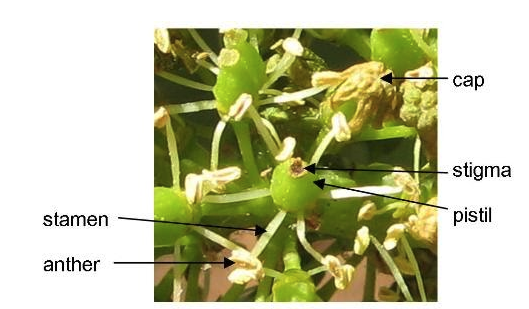
\includegraphics[scale = 0.65]{flowerlabels}
  \caption{The anatomy of winegrape flowers. Source: \href{http://www.extension.org/pages/31097/parts-of-the-grape-vine:-flowers-and-fruit\#.U1f7TeaSy2K} {Hellman 2012} }
  \label{fig:labeledFlowers}
\end{figure}

\begin{figure}
  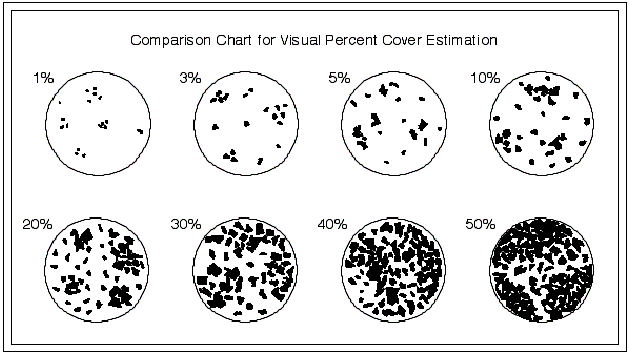
\includegraphics[width=\linewidth]{percentcover}
  \caption{Guide for estimating percent cover. Source: \url{www.nature.nps.gov} }
  \label{fig:percentCover}
\end{figure}

\begin{figure}
  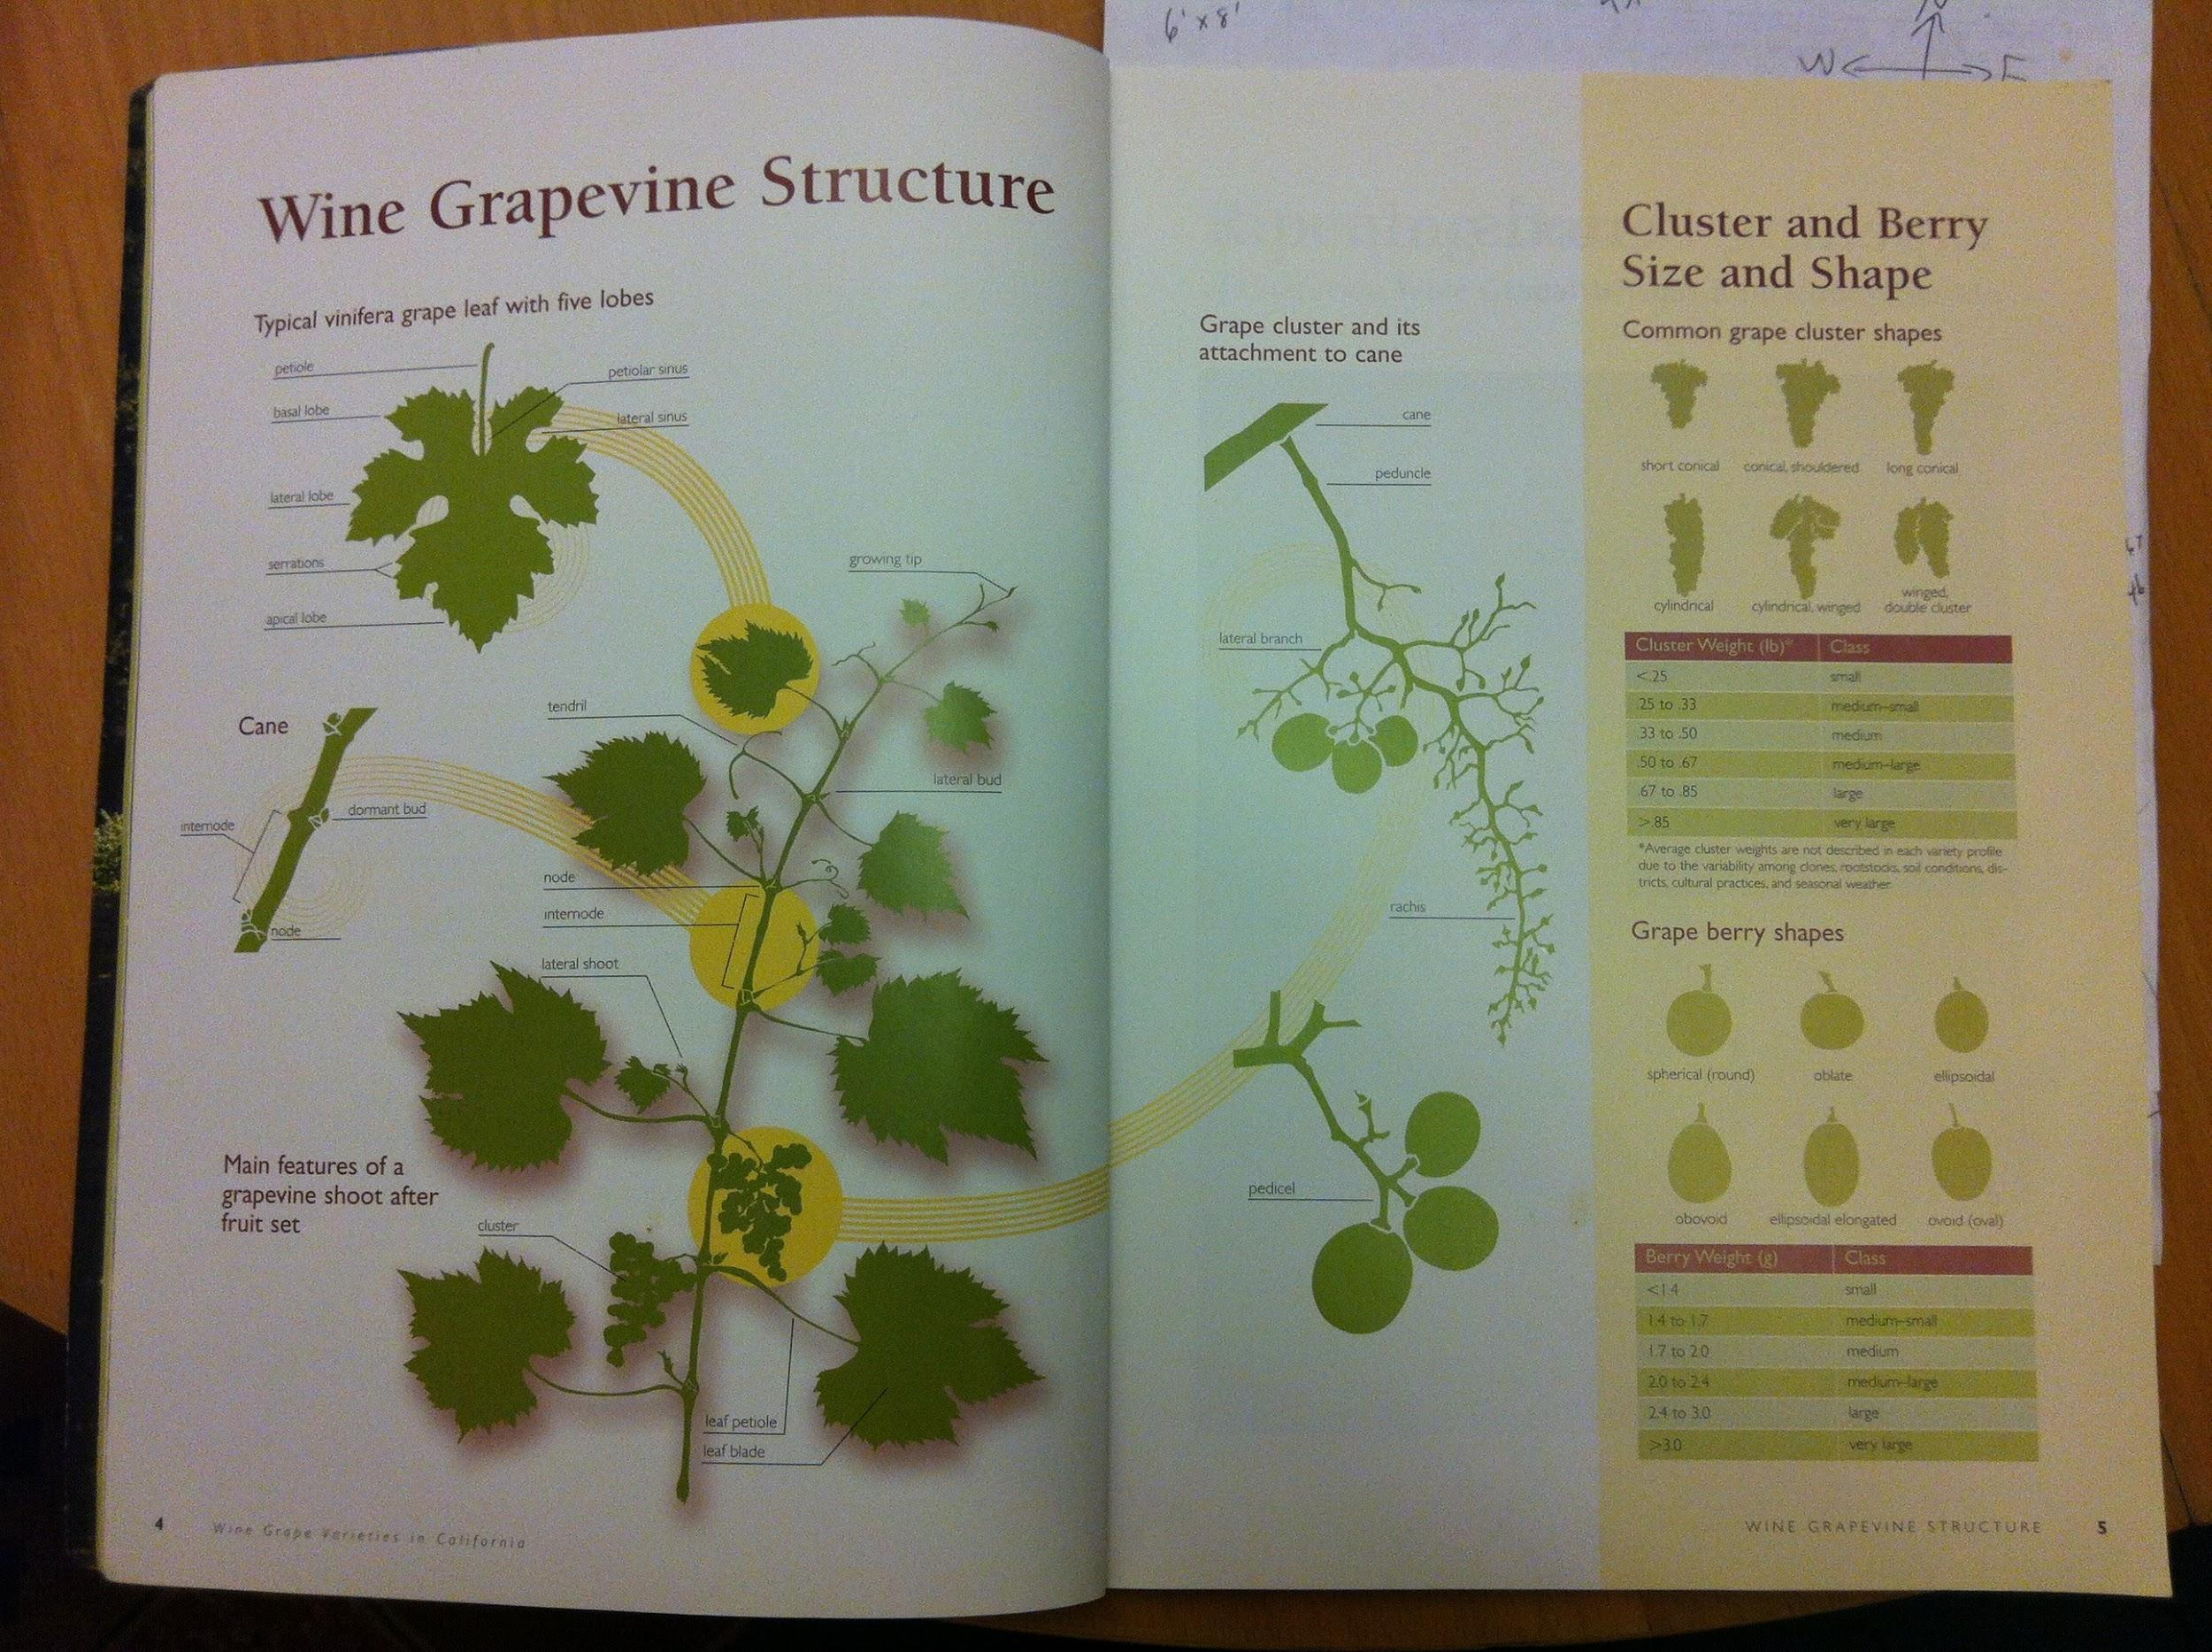
\includegraphics[width=\linewidth]{Bettiga2003Diagram.jpg}
  \caption{An informative diagram of winegrape shoot and berry structure. Source: Bettinga et al., 2003, Wine Grape Varieties in California. }
  \label{fig:Bettiga2003Diagram}
\end{figure}
	
\end{enumerate}

\subsection{Understanding Veraison}
Veraison is a physiological change in the grape where sugar accumulation begins, and the berries begin to enlarge, soften, accumulate sugars and lose acids, and change color (this is quite noticeable in red varieties, and more subtle but still visible in white varieties). At veraison, water transport from the xylem into the berries ends, and the phloem takes over this role.\\ 

Some French colleagues have noted to us that a couple red varieties sometimes become soft before they turn color--and the softness seems to coincide with Brix change. This is about 1-2 out of 50 varieties so it's rare, but try to note softness on red grapes too and if you find any that have changed before color please make a note in the notes field of the datasheet.

According to  to Scott from McIntyre, the earliest variety for them in 2019 was the Sauvignon Blanc in Block C with 50\% veraison on August 9. The berries were tracking behind in 2020.

\section{Brix Sampling}
\subsection{Understanding Ripening (Brix)}

Following the beginning of the ripening process at the onset of veraison (start of rapid accumulation of sugar in the berries detectable as color and softness change), the grape undergoes many changes in the process of ripening, the most obvious of which is the accumulation of sugars and the loss of acids. Sugar accumulation tends to happen at a linear rate, though the slope (rate) of accumulation differs between varieties, and can be influenced by temperature and other vineyard conditions. Traditionally, ripeness was determined by achievement of a certain level of sugar, which is measured in units of degrees Brix (a percentage by weight of sugar, historically 24$^{\circ}$ Brix was considered commercial ripeness on average, though it varies from variety to variety and by wine style). Recent trends have been to harvest later, at a higher degree of ripeness, resulting in higher alcohol wines since the higher sugar levels ferment into more alcohol. \\

Because there can be so much variability in the date of commercial harvest, depending on factors including site, variety, winemaker preference, it is important to measure a quantitative indicator of maturity, rather than to use harvest date or the accumulation of degree-days as phenological markers. Therefore, we will measure Brix at 3-4 dates in the vineyards, with the aim of bracketing the ripening schedule and getting enough data points to plot the ripening trajectory about of different varieties (perhaps between about 18$^{\circ}$ Brix, the level of harvest for sparkling wine styles, to  26$^{\circ}$ Brix or more, the levels commonly found for red wines in California. However, our sampling is based on dates, rather than on desired Brix levels per se). These dates will commence approximately 6 weeks after the onset of veraison, and repeat at approximately 10-day intervals. 

\subsection{Brix Field Methods}

The instrument used to measure sugar in grape juice is a refractometer, which measures how much the light passing through the juice is bent. This angle depends on the degree of soluble solids in the juice- in grapes, nearly all soluble solids (over 90\%) are sugars, thus this is a good measure of sugars. \\

Our goal is to collect a representative sample from throughout the cluster, without taking too many berries to alter the source/sink relations of the cluster, and leaving enough berries to be sampled in subsequent times. We will sample five berries from each of the three flagged clusters on each vine (15 berries per vine). 

\subsubsection{Field Materials}
\begin{smitemize}
\item Small quart-sized freezer plastic Ziploc bags for holding samples of 15 berries per vine, remember freezer-style bags are best!
\item preprinted labels identifying vines from which the samples were taken, stuck on Ziplocs (e.g., the ones we used in 2014 were 1 inch x 2 5/8 inches -- Avery 5160). {\bf Be sure to UPDATE the labels each year} as some individual plants will grow up and join the sampling regime!
\item The above two items (small ziplocs + labels) eventually lead to: {\bf labeled ziplocs} (organized by row inside the last bag for the row*)
\item Sharpie
\item coolers with ice/icepacks and bubblewrap on the ice (so berries don’t touch ice directly). 
\item checklist to make notes on issues you can also make notes directly on Avery labels on the relevant bag, make sure it gets transferred to the electronic notes the next day  when processing samples in the lab (see fieldnotes tab in the spreadsheet for Brix data entry). 
\item clipboard and pen/pencil for checklist
\item camera to photo-document any issues (and note on checklist)
\item latex gloves to keep sticky mess down if you like
\item copy of the most up-to-date protocol
\item flagging tape for reflagging clusters if needed
\item hat, closed toed shoes, sunscreen etc.!

* To organize bags: Put all 10 small ziplocs for one row into the last bag for that row (usually plant 10). Drop the bags at the start of each row.

\end{smitemize}

\subsubsection{Field Protocol}
\begin{enumerate}
\item Sugar levels can vary throughout the day, and increase with temperature. It is therefore important to try to collect berries when they are cool, first thing in the morning! Ideally, sampling will be completed before noon. 

\item You should arrive in the field with the bags all ordered by row.  I suggest setting out the bags for each row in sets of 5-10 rows at a time (I set out 8 at a time). Place the bag of bags at the head of each row cross-checking the row number as you place the bag of bags down (and check again as you start that row); then work through each row. This way if all the bags are gone you know you're all set; be careful that you keep track of any bags you put down as you work through a row (more below). ??? see comment % Maybe organize by block and group. Not sure about leaving them at the end of the rows - doesn't seem logical for the Okanagan vineyards. Is there another organization we could do?

\item For your first 5 and last 5 vines, take an extra sample of 15 berries from the ALTERNATE cordon (not flagged clusters, there are ‘REP’ bags for these, they are not always exactly the first and last five as I maximized variety diversity). We will test these in the lab immediately following field sampling and record the values to compare with those read in the lab the next day, after berries have been refrigerated. The first five samples are used to compare grapes collected when cool to grapes after refrigeration; the last five samples help test the effect of heat (as the day warms up). %For 2017 we actually have TWO REPS per plant so you can do one set of the REPS at the start and the other set as the last grapes you do (that is, after all other grapes are done). %% Would this be at each vineyard?

\item At each vine, collect five berries from each of the three flagged clusters. Clusters generally develop from top to bottom so collect berries from the approximate positions indicated in Figure \ref{fig:conecluster}. Try to close or avert your eyes and sample by feel to avoid being visually drawn to the most developed grapes. Healthy grapes should feel firm and juicy to the touch. A very squishy or disintegrating grape is diseased and should be avoided. Do your best to pull or twist the grape from the rachis while keeping it relatively intact (it will store better until measurement)- but sometimes, on tightly packed clusters, it’s impossible to extract 15 whole berries without breaking them. 

Unless of course your berry cluster is not the classic ‘conical’ shape (see ‘short conical’ and ‘long conical’ from berry cluster Figure \ref{fig:clustershapes} below). If you have a conical cluster with strong shoulders or cylindrical winged, take an extra berry from the top and one less from the middle, for cylindrical take your five berries spaced relatively evenly from top to bottom and so on so you’re getting a good spacing of berries, representative of the total cluster shape. In extreme cases where you’re not sure what to do you can take 5 berries from the middle.

\begin{figure} [h]
  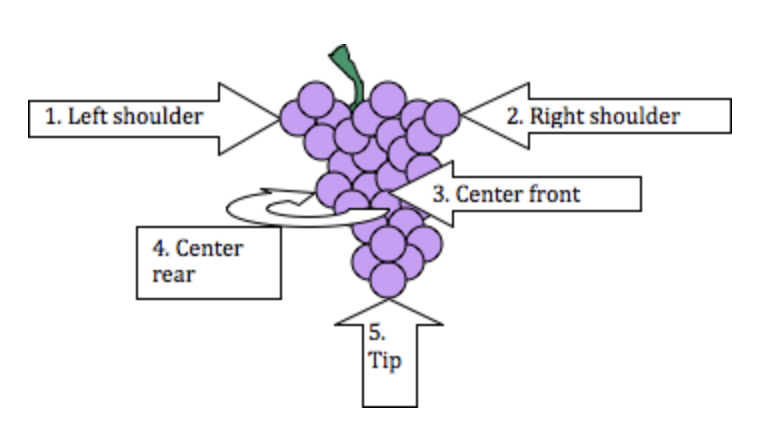
\includegraphics[scale = .75]{conecluster.png}
  \caption{Sampling locations on cluster }
  \label{fig:conecluster}
\end{figure}

\begin{figure} [h]
  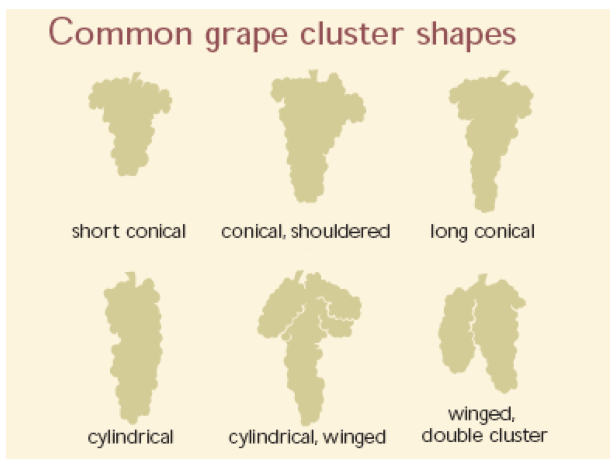
\includegraphics[scale = .75]{clustershapes}
  \caption{Berry cluster shapes. Figure stolen from ‘Wine Grapevine Structure’ online.}
  \label{fig:clustershapes}
\end{figure}

\item Problem clusters: sometimes a flagged cluster will be missing, rotten, undeveloped, shriveled, or otherwise messed up. Such clusters are likely to have anomalous Brix readings. If there is a normal, healthy-looking cluster nearby, remove the flag from the bad cluster, flag and sample the healthy cluster. (However, note that you should only take berries from a “count” cluster, that is, one that arises from one of the first four nodes of the cane. Some varieties of grapevines develop a “second crop” of clusters that are borne from much higher in the cane, and are generally much smaller and much less ripe than the main clusters. These are not representative of the normal developmental and ripening trajectory, so should not be sampled.)  If all clusters on a vine are similarly problematic, but there are enough healthy-appearing grapes to sample 5 grapes from a cluster, sample and flag that cluster. Remember that our unit of analysis is the vine (not cluster), so we are better off getting a healthy, representative sample from a vine if it is possible. If all available grapes are seriously deformed or rotten, note this and do not sample. %See table 2 below.

You should have a clipboard to keep a note of any issues you run into. In later sampling dates you should also note any plants where berries appear {\bf past-maturation and beginning to shrivel} (however, as long as the grapes appear to have developed properly and are only shriveling due to being on the vine too long you should still sample the plant -- once you cannot get juice from the berries then do not sample). {\bf Take photos as necessary to document issues or how you are noting shrivel.}

A rule of thumb in guiding whether to sample is to make a scale of 1-4 for berry shrivel and for rot, in each case score them as follows: \\
4: $>$75\% of berries on plant are in this state \\
3: 50-75\% of berries on plant are in this state \\
2: 25-50\% of berries on plant are in this state \\
1: $<$25\% of berries on plant are in this state \\
Add your two scores (one for rot and one for shrivel) -- if the total is 4 or higher, don't sample. {\bf Write down the score for each (shrivel, rot)! (Update data entry sheet to have a column for shrivel, and a column for rot.)}

\item Place the 15 berries from one vine in the labelled ziploc. While working one row you can either (1) put each bag next to each plant or (2) create one or two centralized stacks of bags (in the shade as much as possible); either way collect all 10 bags when you finish a row and put them directly in the cooler. Try to have a layer of something (cardboard, plastic bags, bubble wrap) so grapes don’t touch ice directly. 

\item When all berries have been collected, store in the refrigerator overnight or directly package and ship to Vancouver % take to the lab and -- for most berries (but see step 8) -- refrigerate overnight (up to a few days max) before beginning the lab protocol to measure Brix, or else start reading directly if you have time. 

%Remember to read the Brix levels immediately on arrival in the lab on the first and last 5 samples collected from the alternate cordon (the REP samples), for comparison with the results from the main (flagged) cordon, which will be read with all the others during the main lab work day. %%%%% Should this go to lab? How should we adapt this to labwork at UBC?

\item Transcribe all info from your field checklist into the 'field\_notes' tab of the brix\_dataentry google doc. Also transcribe your time in and out of the field. 

\end{enumerate}

{\bf When to stop measuring Brix?}
So, you skip sampling when all the main crop of berries are destroyed by birds, are all diseased or shriveled or are oddly undeveloped. But when else do you stop measuring Brix? Two options:
\begin{enumerate}
\item The Brix measurement on the previous sampling date was 30 degrees or higher.
\item The Brix measurement on two consecutive sampling dates was less than 0.1 Brix different for that exact plant (but ask Lizzie to take a look at any you want to skip for this reason).
\end{enumerate}

{\bf Shipping grapes to UBC}

Package grapes in styrofoam freezer box and place in a cardboard box for shipping. \\ %With ice pack?

Use the following accounts for shipping: \\
Purolator Acct \# - 1154218 \\
FedEx Acct \# - 143080285 \\

Address the package to: \\
Elizabeth Wolkovich \\
Forest and Conservation Sciences \\
University of British Columbia \\
3041 - 2424 Main Mall \\
Vancouver, BC V6T 1Z4 \\

\subsection{Brix Lab Methods}
Berries will be shipped back to Vancouver so labwork can be done in the Wolkovich Lab, Forest Sciences Center

\subsubsection{Labwork Materials}
\begin{smitemize}
\item refractometer %Lizzie will add brand and make
\item Distilled water in a squeeze bottle for rinsing refractometer between samples
\item Kimwipes for wiping off refractometer between samples
\item Pipettes for applying grape juice to refractometer 
\item Data sheet for recording Brix (electronic, %see brix_dataentry on google drive in ‘Brix’ folder in RMI data)
\item Deionized (aka Distilled) water (for zeroing refractometer)

\end{smitemize}

\subsubsection{Lab Protocol}
\begin{enumerate}
\item Put the berries in the fridge (not freezer). Label them with your name, the date that you put them in, and the date that you will be done.
\item Set up and calibrate refractometer with DI water as a blank. Make sure temperature compensation is on. 
\item Take a ziploc containing 15 berries from the cooler. Manually crush the berries so that the juice is released from all berries and well-mixed inside the bag. 
\item Use a pipette (with a disposable tip) to add juice on the prism, covering the prism. %is it a specific amount? % In the past we have used plastic spoons, which we rinsed and wiped with Kimwipes between each use. 
\item Read and record Brix on data sheet (or direct entry into tablet).   
\item Use Kimwipe to remove juice sample from prism. 
\item Squirt prism with distilled water and wipe off with another Kimwipe. 
\item Repeat. 
\item At the end of the day, please take the trash out that has the berry bags in it; this helps prevent fruit flies.
\end{enumerate}

It’s helpful to crush ~20 bags of berries at a time to speed up the entire process while working alone. % once you crush them, do you need to keep them cool until you measure?

Time estimates: Lizzie working alone up to max speed did 40 samples an hour -- so for 2014 probably best to estimate 9-10 person hours. Sadie working alone took about 12-13 total hours start to finish for measuring brix and 5 hours collecting berries. 

\section{Contacting vineyards}
Please ask Mira and/or Faith to introduce you before reaching out to these folks! If you have any issues, let us know.\\

Quails' Gate (Chad) asked that we contact them two days prior to working in the vineyard for permission but Judy told April Mahovlic that texting the day before is fine. Arterra prefers to give permission the day before we want to work in the vineyard because they have flexible management and may make management decisions quickly. We have been texting for permission once you have been introduced. It might be good to call the first time you contact the managers. \\

%Sebastian Farms
%Rob Achurch (250) 490-6162
%Devin Methvin (250) 462-0662
%rachurch@sebastianfarms.ca
%dmethven@sebastianfarms.ca

{\bf Quails' Gate}

Head Viticulturalist: Chad Douglas (250) 317-3006 (Chad Douglas, Quails Gate as of 2020), Email: Chad@sfewine.com (cdouglas@quailsgate.com)

Assistant Manager for Quails' Gate Estate and Mannhardt vineyards is Judy Wanbon (250)-317-8305 (email: Jwanbon@quailsgate.com) \\

{\bf Arterra}

Dark Horse contact and Head Viticulturalist %are these the right titles?

Mike Watson (250) 498-9391

mike.watson@arterracanada.com\\
% add Tamara's contact info?

Nk'Mip Cellars --

Nelson Dutra - Vineyard Manager

250.485.8085 (Email: nelson.dutra@arterracanada.com) \\

McIntyre and Whitetail -- 

Contact FIRST is the vineyard supervisor:

Scott Carlson 250.485.7920 (Email: scott.carlson@arterracanada.com)

Vineyard Manager is Manjit Deol: 250.485.8215


\section{Site Directions and Access}

{\bf Quails' Gate: Main Estate vineyards} \\
The main Quails' Gate vineyard is easy to find using Google Maps if you use the Quails' Gate Wineshop as the destination. 
From BC-97 North, turn right onto Gellatly Rd then left on Boucherie Rd. Quails' Gate Wineshop is about 5.5 km up the road. The parking lot for the main vineyard is a little bit before the Wineshop and is labeled with a "Staff Parking Only" sign (see Figure \ref{fig:QGparkingLot}. You can park here for the upper and lower vineyards (just across the road). We do not drive in the estate vineyards.

\begin{figure} [h]
  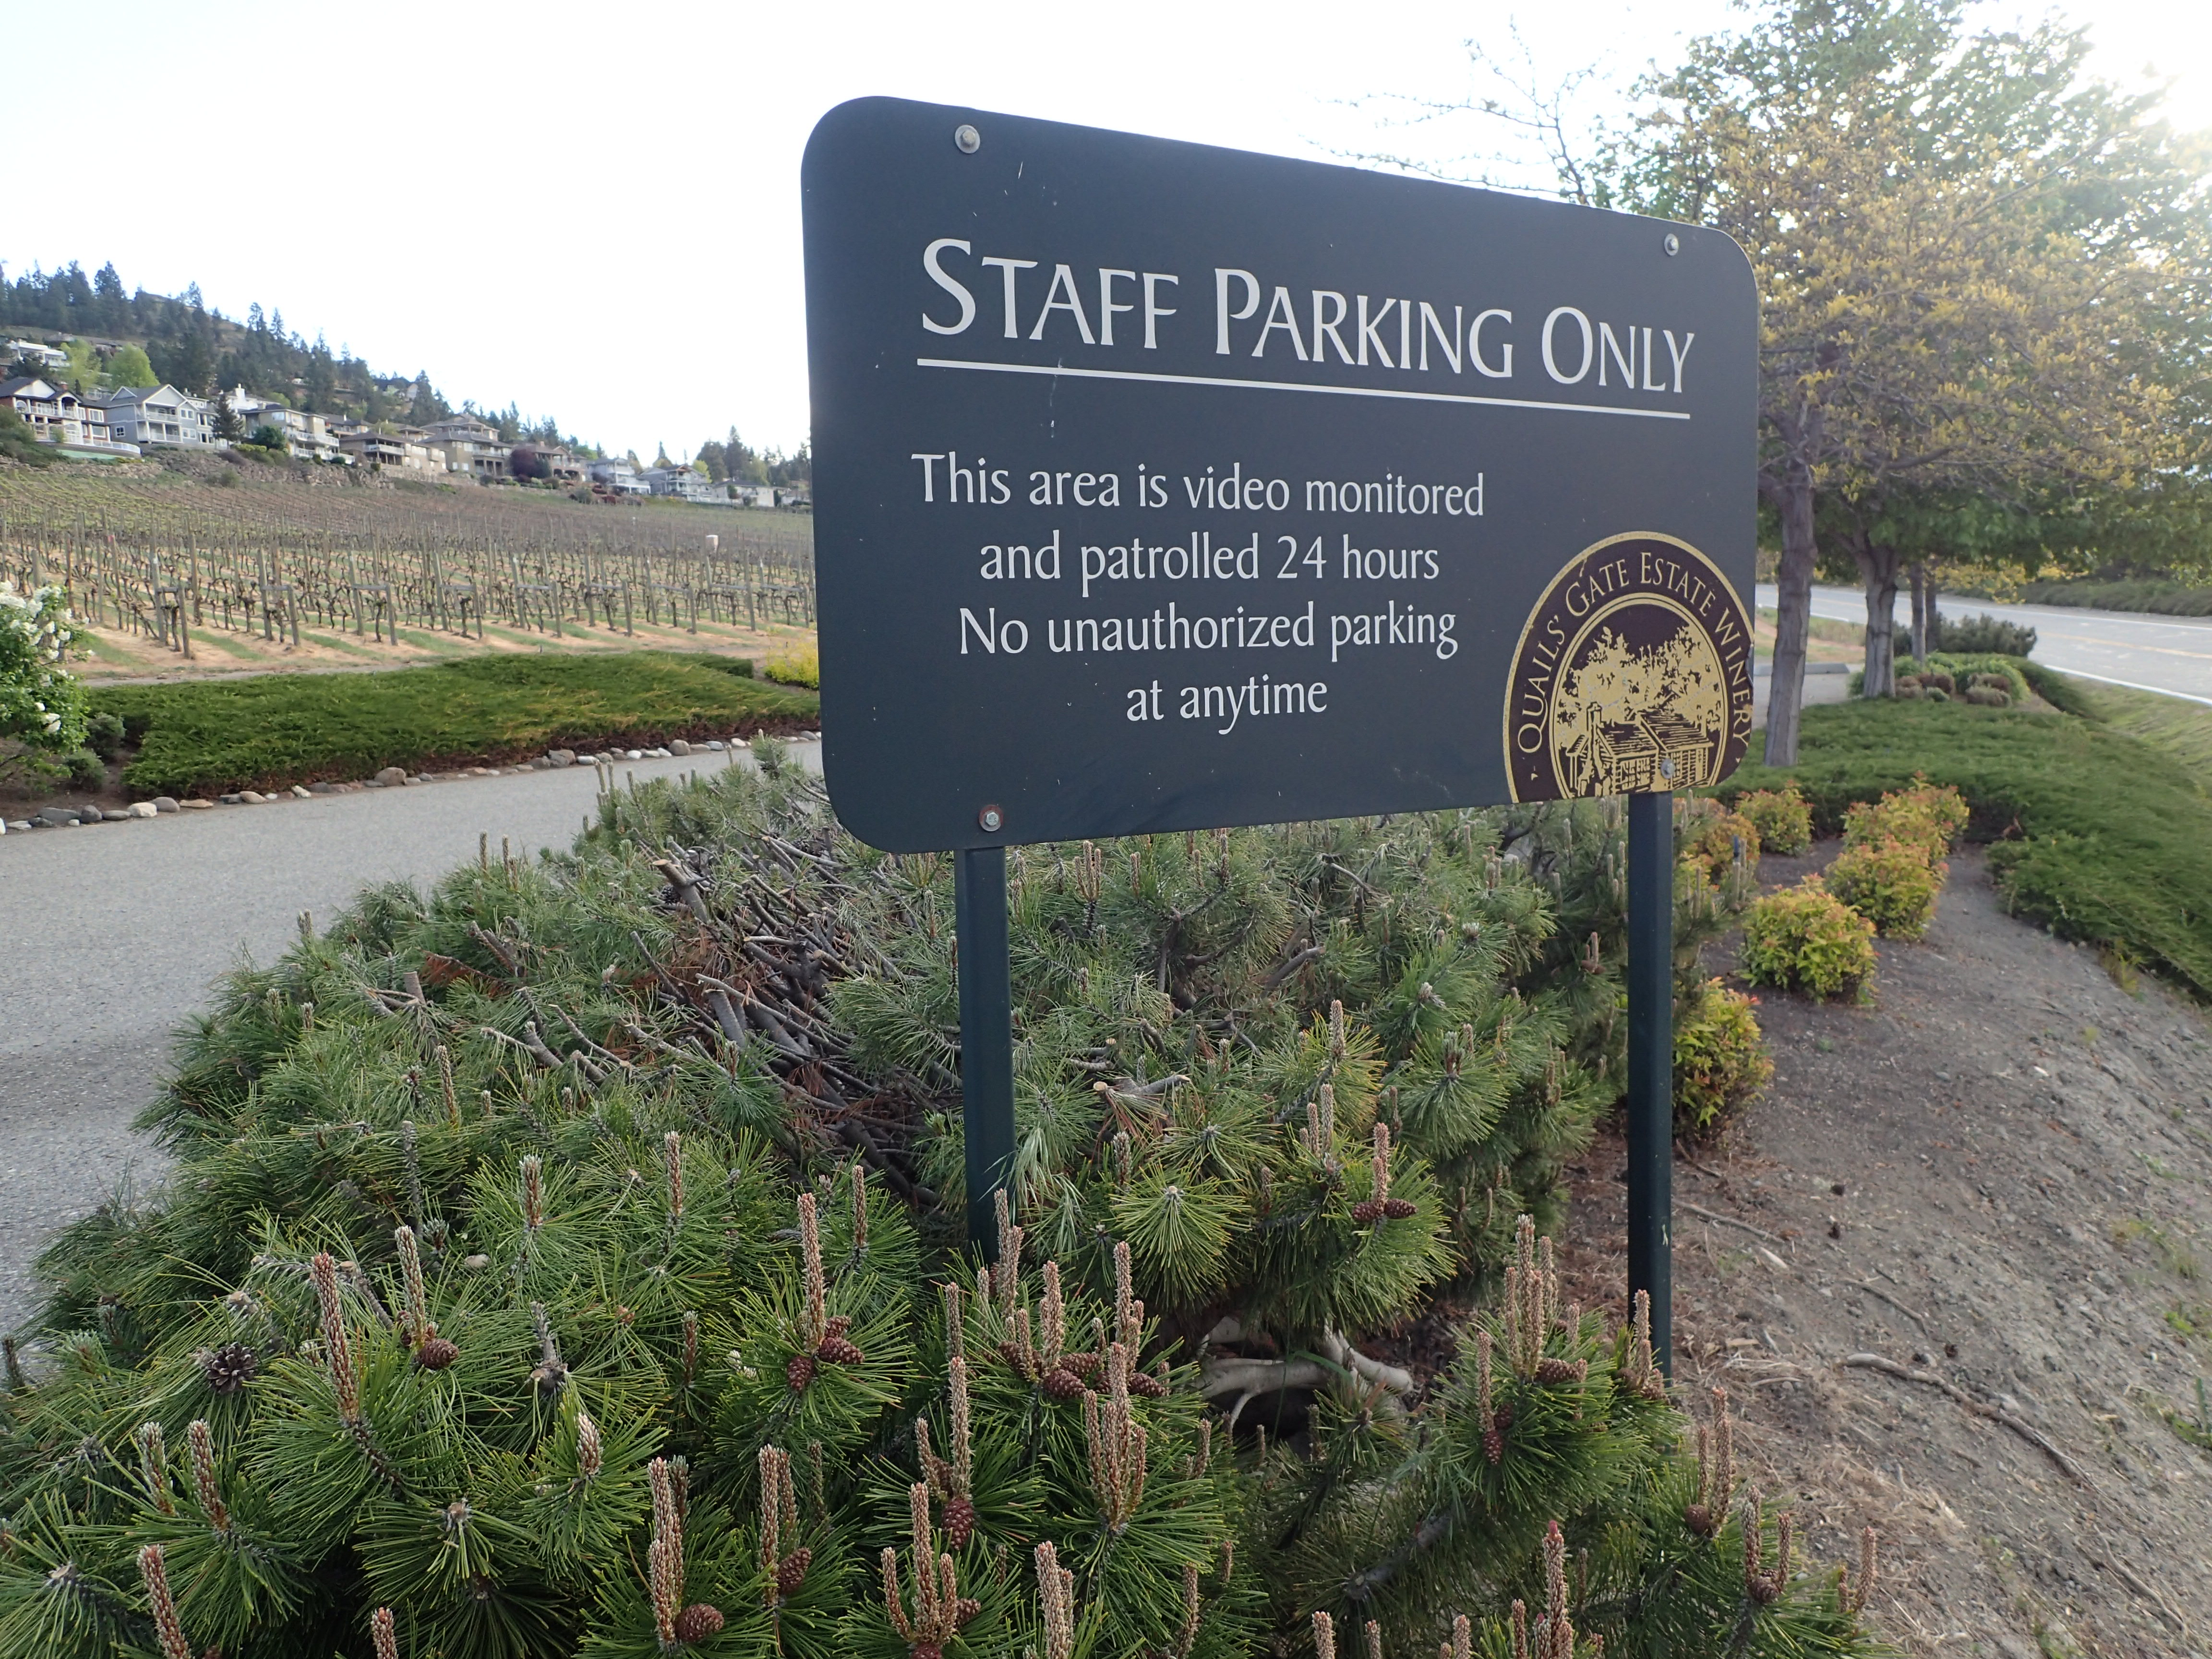
\includegraphics[scale = .25]{qgParkingLot.JPG}
  \caption{The sign marking the vineyard parking lot }
  \label{fig:QGparkingLot}
\end{figure}

There is no gate to the parking lot and no gate to prevent people from walking through the vineyard so as long as you have permission from Judy Wanbon to be in the vineyard, access at any time is easy. \\

{\bf Quails' Gate: Mannhardt Vineyard} \\
Mannhardt Vineyard is close to Quails' Gate. From Boucherie Rd, turn right on to Sunnyside Rd (turn is just after the Wineshop parking lot), left at the stop sign to Kelly Dr, and right at Aubrey Rd. Turning right on Aubrey essentially takes you into the vineyard. We have been driving around this vineyard.

Mannhardt does not seem to be gated. Technically, there is a gate but it has never been closed when we are there and non-vineyard people often walk through the site. You should only need permission from Judy and should be able to access it at any time. \\

{\bf Arterra: NK'MIP Cellars} \\
This site is easy to find using Google Maps if you set NK'MIP Cellars as the destination.
From BC-97 South, turn left on BC-3 E/Main Street and left onto 45 St. The 45 St corner has a Petro-Canada and a sign for NK'MIP Resort. Follow this road up to the resort and once in the resort parking lot, turn right and follow the road passed the sculpture of the turtle and man to the parking lot on the left. Across the road you should see the NK'MIP Cellars building and a garage/equipment shed. 

One section of the vineyard is at along the parking lot. The main vineyard is across the road - the gate is between the winery building and equipment shed. There is an additional gate from the resort parking lot that is obvious and decorative. I think it is best to use the other gates if possible. The spray board is on the equipment shed.

Mike Watson gave us a key that opened both gates to be returned at the end of the season. Get permission from Nelson Dutra to be in the vineyard. \\

{\bf Arterra: Dark Horse} \\
Easy to find with Google Maps if you set the destination to 4859 Mariposa Rd, Okanagan-Similkameen C, BC.
From BC-97 South, turn right onto Rd 11 then left on Mariposa Rd. You should see the main office building and parking lot behind a hedge right after the turn. Across the road from the parking lot are blocks 1 and 2. Driving around these will take you to an exit at the intersection of Mariposa Rd and Rd 11.

Following the paved road passed the office will take you up the hill to the other blocks. There are signs marking Dark Horse (Figure  \ref{fig:DHsigns}). The spray board is on the side of the equipment shed.

I do not think the vineyard itself is gated - it has always been open when we arrive if it is. We will check this next time we are there. Get permission from Mike Watson but always check the spray board before starting work. \\

\begin{figure} [h]
  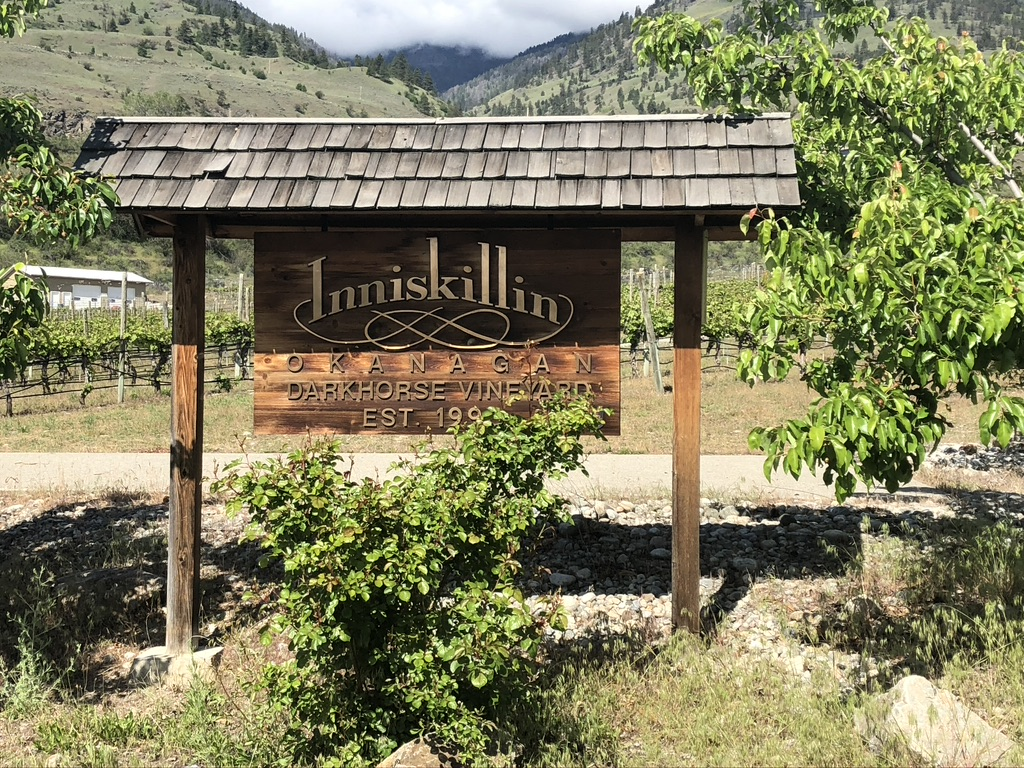
\includegraphics[scale = .25]{darkhorseSign1.jpeg}
   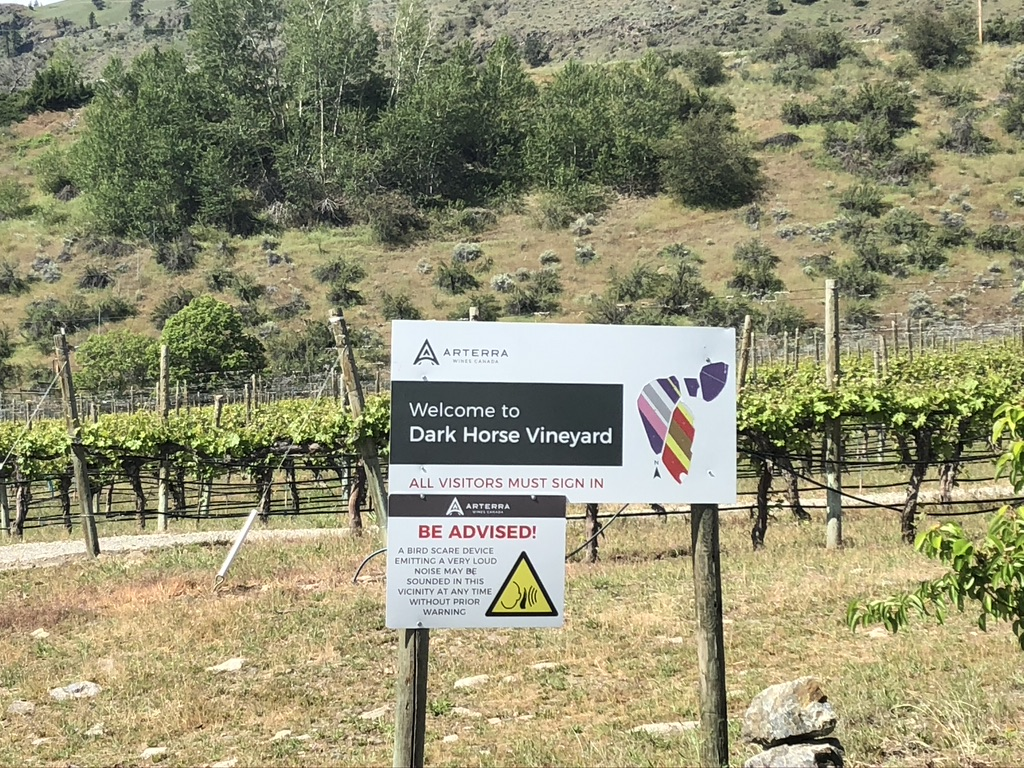
\includegraphics[scale = .25]{darkhorseSign2.jpeg}
  \caption{The signs marking the entrance to Dark Horse Vineyard}
  \label{fig:DHsigns}
\end{figure}

{\bf Arterra: McIntyre} \\
Can use 4181-4101 McKinney Rd, Oliver, BC V0H 1T0 to search on Google Maps.
From BC-97 South, turn left on Tucelnuit Dr (Jackson Triggs winery is on the corner) continue until the road ends at McKinney Rd. Turn left onto McKinney Rd and follow it for about 1 km until you see McIntyre vineyard on the left. You will have to drive up the hill to get to the vineyard. The office is on the opposite side of the vineyard.

There is another exit/entrance on Arrow Head Rd between blocks A and C. Turning right out of block C (left from A) will take you out to McKinney Rd where you take a left and drive passed the main entrance to return to Tucelnuit Dr.

Get permission to be in the vineyard from Scott Carlson - he will tell you when they have sprayed. There should also be a spray board on the office according to Mike Watson. \\

% {\bf Arterra: Whitetail} \\
% Can use 34401 Black Sage Rd, Oliver, BC V0H 1T0 to search on Google Maps.
% From BC-97 South, turn left on Tucelnuit Dr (Jackson Triggs winery is on the corner) continue until the road ends at McKinney Rd. Turn left on McKinney Rd and a quick right to Black Sage Rd (you are essentially going straight but you have to change streets). Follow Black Sage Rd until you see the sign for Whitetail. 

% You will enter into the main vineyard where you will find blocks C and D. There is another part of the vineyard with block B to the north, just across an empty field. If you follow the road to the hill, there is a road up the hill to block J on the top of the bench. To reach block F, you have to exit the main vineyard - turn left onto Black Sage Rd and take the first right onto Nk'Mip Rd. The vineyard with block F is the first right on this road. There are multiple exits back onto Black Sage Rd.

% Get permission to be in the vineyard from Scott Carlson - he will tell you when they have sprayed. There should also be a spray board on the office according to Mike Watson. \\


\section{Vineyard Management}
What we know about how the vineyards are managed can be added here
\subsection{Pest Management}
{\bf McIntyre} \\ % and Whitetail 
From Scott:
"We generally spray preventively for Mildew and only on a as necessary basis for pests such as leafhopper or cutworms. Mildew sprays start at 3 leaf stage and then go on the recommended spray interval based on each chemical. \\

At Arterra we generally spray:

3 leaf stage – Kumulus and then 10-14 days after that depending on weather (rain/humidity) until full flowering and cap fall.

Then we apply systemics such as Nova, Flint, Sovran, Inspire Super, and various other ones, always changing groups, until veraison. From there we generally spray 1 to 2 more Kumulus sprays just to control canopy mildew leading into harvest/dormancy." \\

{\bf Dark Horse} \\
From Tamara:

"Cutworms: We monitor for bud damage in April and early May, and spray Altacor once only in the blocks/sections with damage significantly above our economic threshold (around 5\% damage). Last year we tried using Intrepid, but found that the control efficacy was much lower than that of Altacor so we do not plan to continue using it. \\

Weeds: All our blocks are typically treated with a combination of Roundup and Chateau in early/mid April. For blocks with higher weed pressure, they may be treated again later in the season (June-August) with either Ignite or a second glyphosate spray (Roundup or Touchdown) depending on the weeds present. \\

Powdery Mildew: We typically apply Kumulus early in the season as a preventative spray, starting in late April/early May (around 5-10cm shoot growth) and applied at approximately 14-day intervals for 2-3 applications. After that we will switch to 2-3 applications of local systemic sprays at 14-day intervals, alternating pesticide group numbers as much as possible. Some of the sprays we have used for this in recent years include Quintec, Property, Fullback, and Vivando. We plan to incorporate Cevya into our rotation this year as well. We finish off our season with 2 more Kumulus sprays. For blocks with historically high mildew pressure, we will often add a Lime Sulphur spray in early April (pre-budbreak). \\

Erineum Mite: For blocks with high erineum mite pressure in the past, we will consider treating in early April (pre-budbreak) with Lime Sulphur or a high rate of Kumulus. \\

Leafhopper: We actively monitor for nymphs, adults, and eggs, and only treat the blocks or sections of blocks with high leafhopper pressure. If necessary, we spray during the nymph stage, usually in the 1st generation (July), and typically use Clutch or Sivanto Prime. \\

Botrytis: We only treat blocks with high botrytis pressure in the past, or blocks showing symptoms of botrytis. In the past we have used Switch, Elevate, Scala, Fracture, and Serifel. Sprays are usually applied in June or July, but we will occasionally use Fracture or Serifel to treat blocks closer to harvest (September) if needed. \\

Mealybug: We don’t usually treat for mealybug since the population levels don’t normally become large enough to pose a problem in our vineyards, but last year was a bad year for mealybug. We closely monitored mealybug population sizes and used Movento in July to treat blocks with substantially large populations."

{\bf Quails' Gate}
They spray all the vineyards over 3 consecutive days if possible.


\section{Glossary}

\begin{smitemize}
\item {\bf vine}: an individual plant of \emph{Vitis vinifera}. 
\item {\bf permanent part of the vine}: vine parts which are not pruned, and persist from year to year (ex: trunk and cordons).
\item {\bf cordon}: parts of the vine that extend horizontally from the trunk, parallel to the ground, along a horizontal training wire in the trellis. (See Figure \ref{fig:CordonPruned}) They are a permanent part of the vine, may be many years old, and develop bark. 
\item {\bf arm}: a vertical permanent protuberance with bark arising from a cordon. Age three or more years. (Labeled in Figures \ref{fig:CordonPruned} \& \ref{fig:TwoSpurs}). Arms are also called {\bf 'positions'} on the grapevine, as they are selected and maintained to have good spacing, light, and airflow through the canopy, etc. 
\item {\bf cane}: developed shoots grown this year ('one-year-old' by the end of the growing season). Over the course of the season, this year's leaves and clusters grow from buds on the cane. There are differences in terms of cane management between cordon pruned vines (Figure \ref{fig:CordonPruned}) and cane pruned vines (Figure \ref{fig:CanePruned}).
\begin{smitemize}
\item {\bf For cordon pruned vines:} At the end of the season when the cordon pruned vines are pruned, a section of one cane on each arm from last year is retained (this will become a {\bf spur}). This cane is cut to two buds on a vine of average vigor, one bud on a weak vine, and three on a strong vine, to match the growing points to the vine's capacity. The two buds kept will become next year's canes. The second cane (which grew from the upper bud kept from last year) is removed during pruning (Figure \ref{fig:TwoSpurs}). 
\item {\bf For cane pruned vines:} a single full cane is retained at the end of each growing season to serve as bud for the following year (Figure \ref{fig:CaneCrossing}). This cane will be removed at the end of the second growing season so a new cane can take its place. Extra canes may be retained at the head of the trunk to serve as a source of next year's cane. 
\end{smitemize}
\item {\bf spur}: two-year-old wood (meaning, what is left of last year's canes). This will be cut in pruning to retain just the lowest buds. (Labeled in Figure \ref{fig:CanePruned}).
\item {\bf buds}: the compound buds, occurring at nodes, from which this year's growth will happen. This year's shoots will turn into canes, which will eventually bear leaves and clusters. Each of the buds marked 'buds for monitoring' in Figure \ref{fig:TwoSpurs} are what will go through budburst. These bud should be monitored for EL stages numbers 1-15, which refer to the vegetative part of the plant (leaves or shoots), not the reproductive part (clusters). 
\item {\bf cluster}: (AKA {\bf bunch} for table grapes when ripe; AKA {\bf inflorescence}, botanically)-- the fruit of the grapevine, consisting of many berries attached to a {\bf rachis} (the skeleton left behind after you eat a bunch of grapes). The cluster consists of many flowers, which bloom and go through {\bf set} (pollination), in the process shedding their {\bf 'cap'} covering the flowers. Flowers that have set go on to ripen into fruit, the individual berries on the cluster. Clusters are found on the 2nd and 3rd nodes (fruitful nodes) of a cane that grew this year from one of the two buds originally retained at pruning.
\end{smitemize}


\section{Misc}
Tape colors for QG are orange and blue, avoid flagging with these colors\\
Avoid orange and pink for Arterra - they seems to use of have most colors in their vineyards though\\
Ask vineyards at beginning of the season what color they prefer we use

\clearpage
\section{Vineyard Maps}
Below are maps of the vineyards marked with locations marked for the vines we are monitoring.

\begin{figure} [h!]
   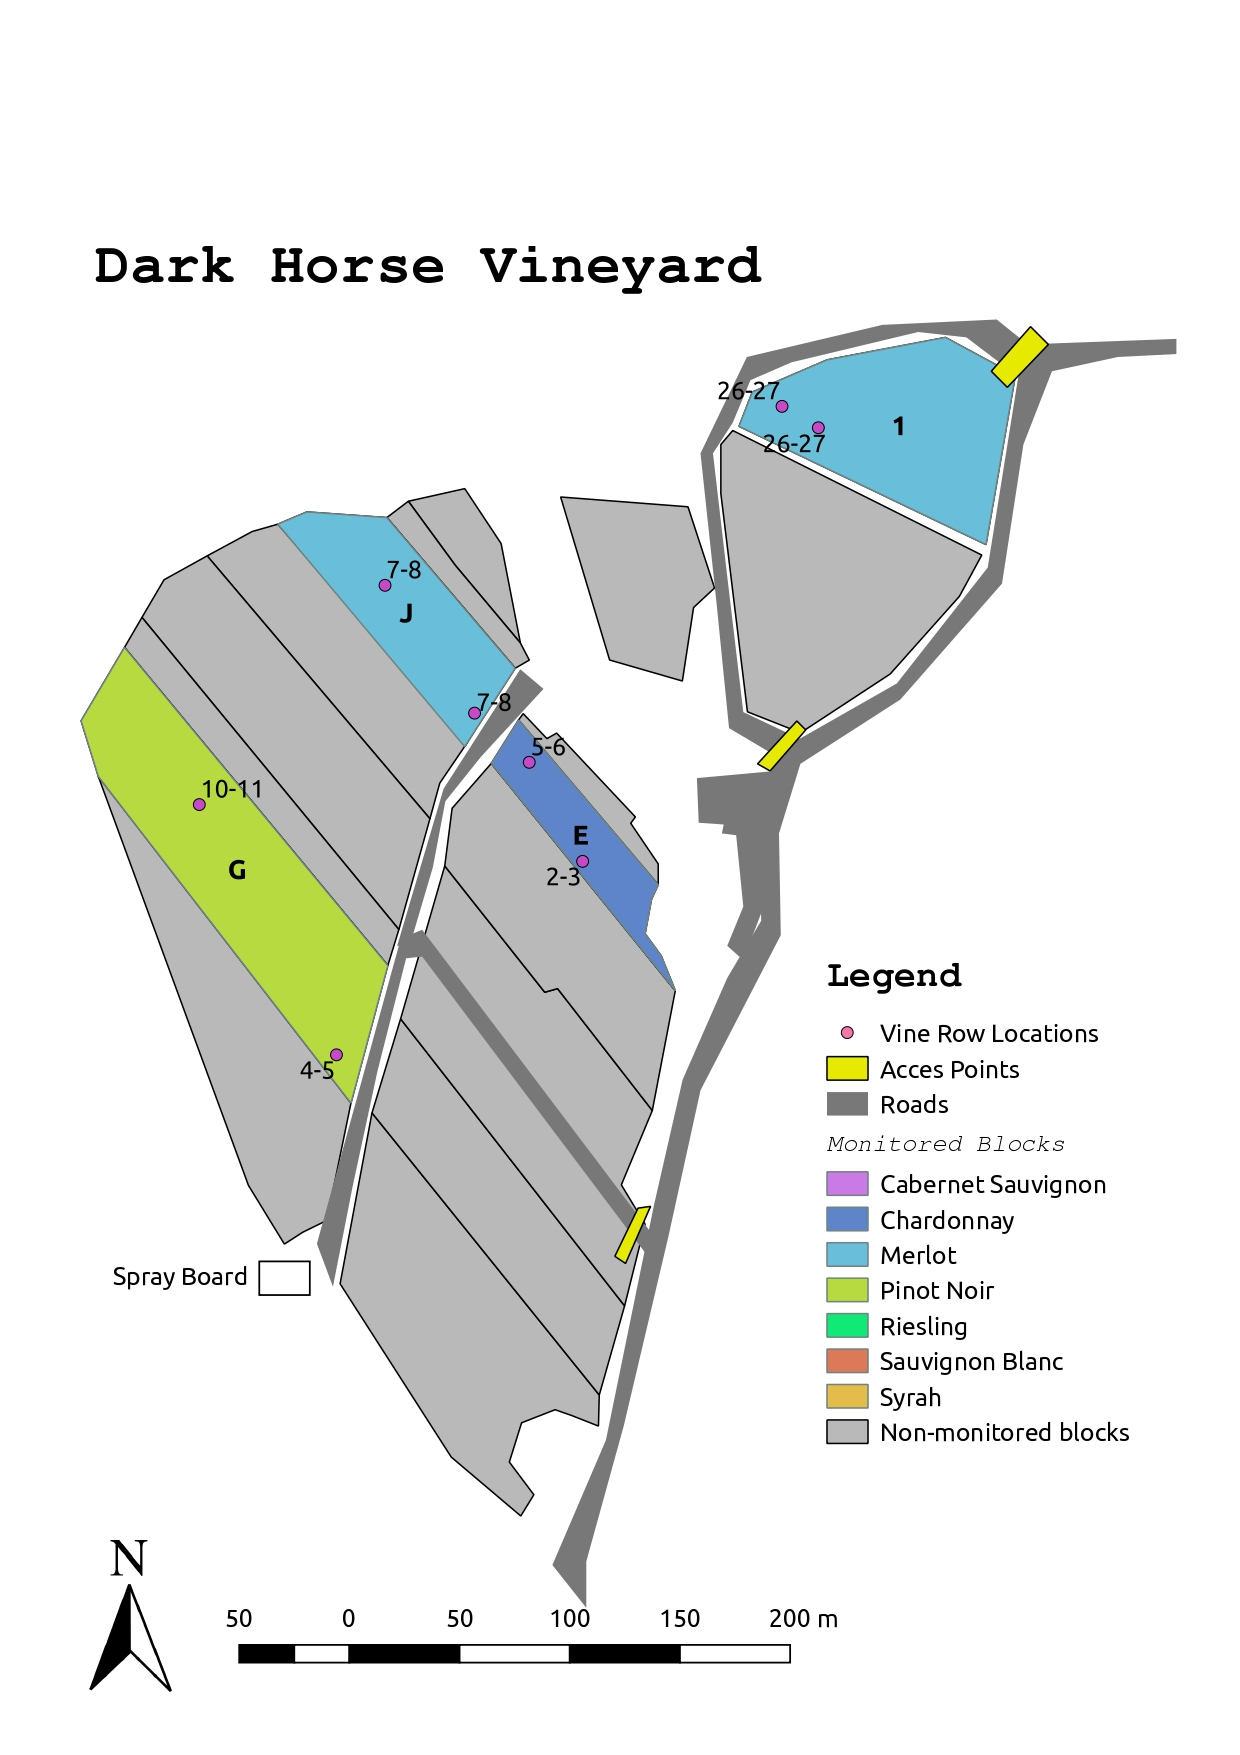
\includegraphics[width = \linewidth]{DH_map.jpg}
  \caption{Map of Dark Horse Vineyard}
  \label{fig:DHmap}
\end{figure}

\begin{figure} [h]
   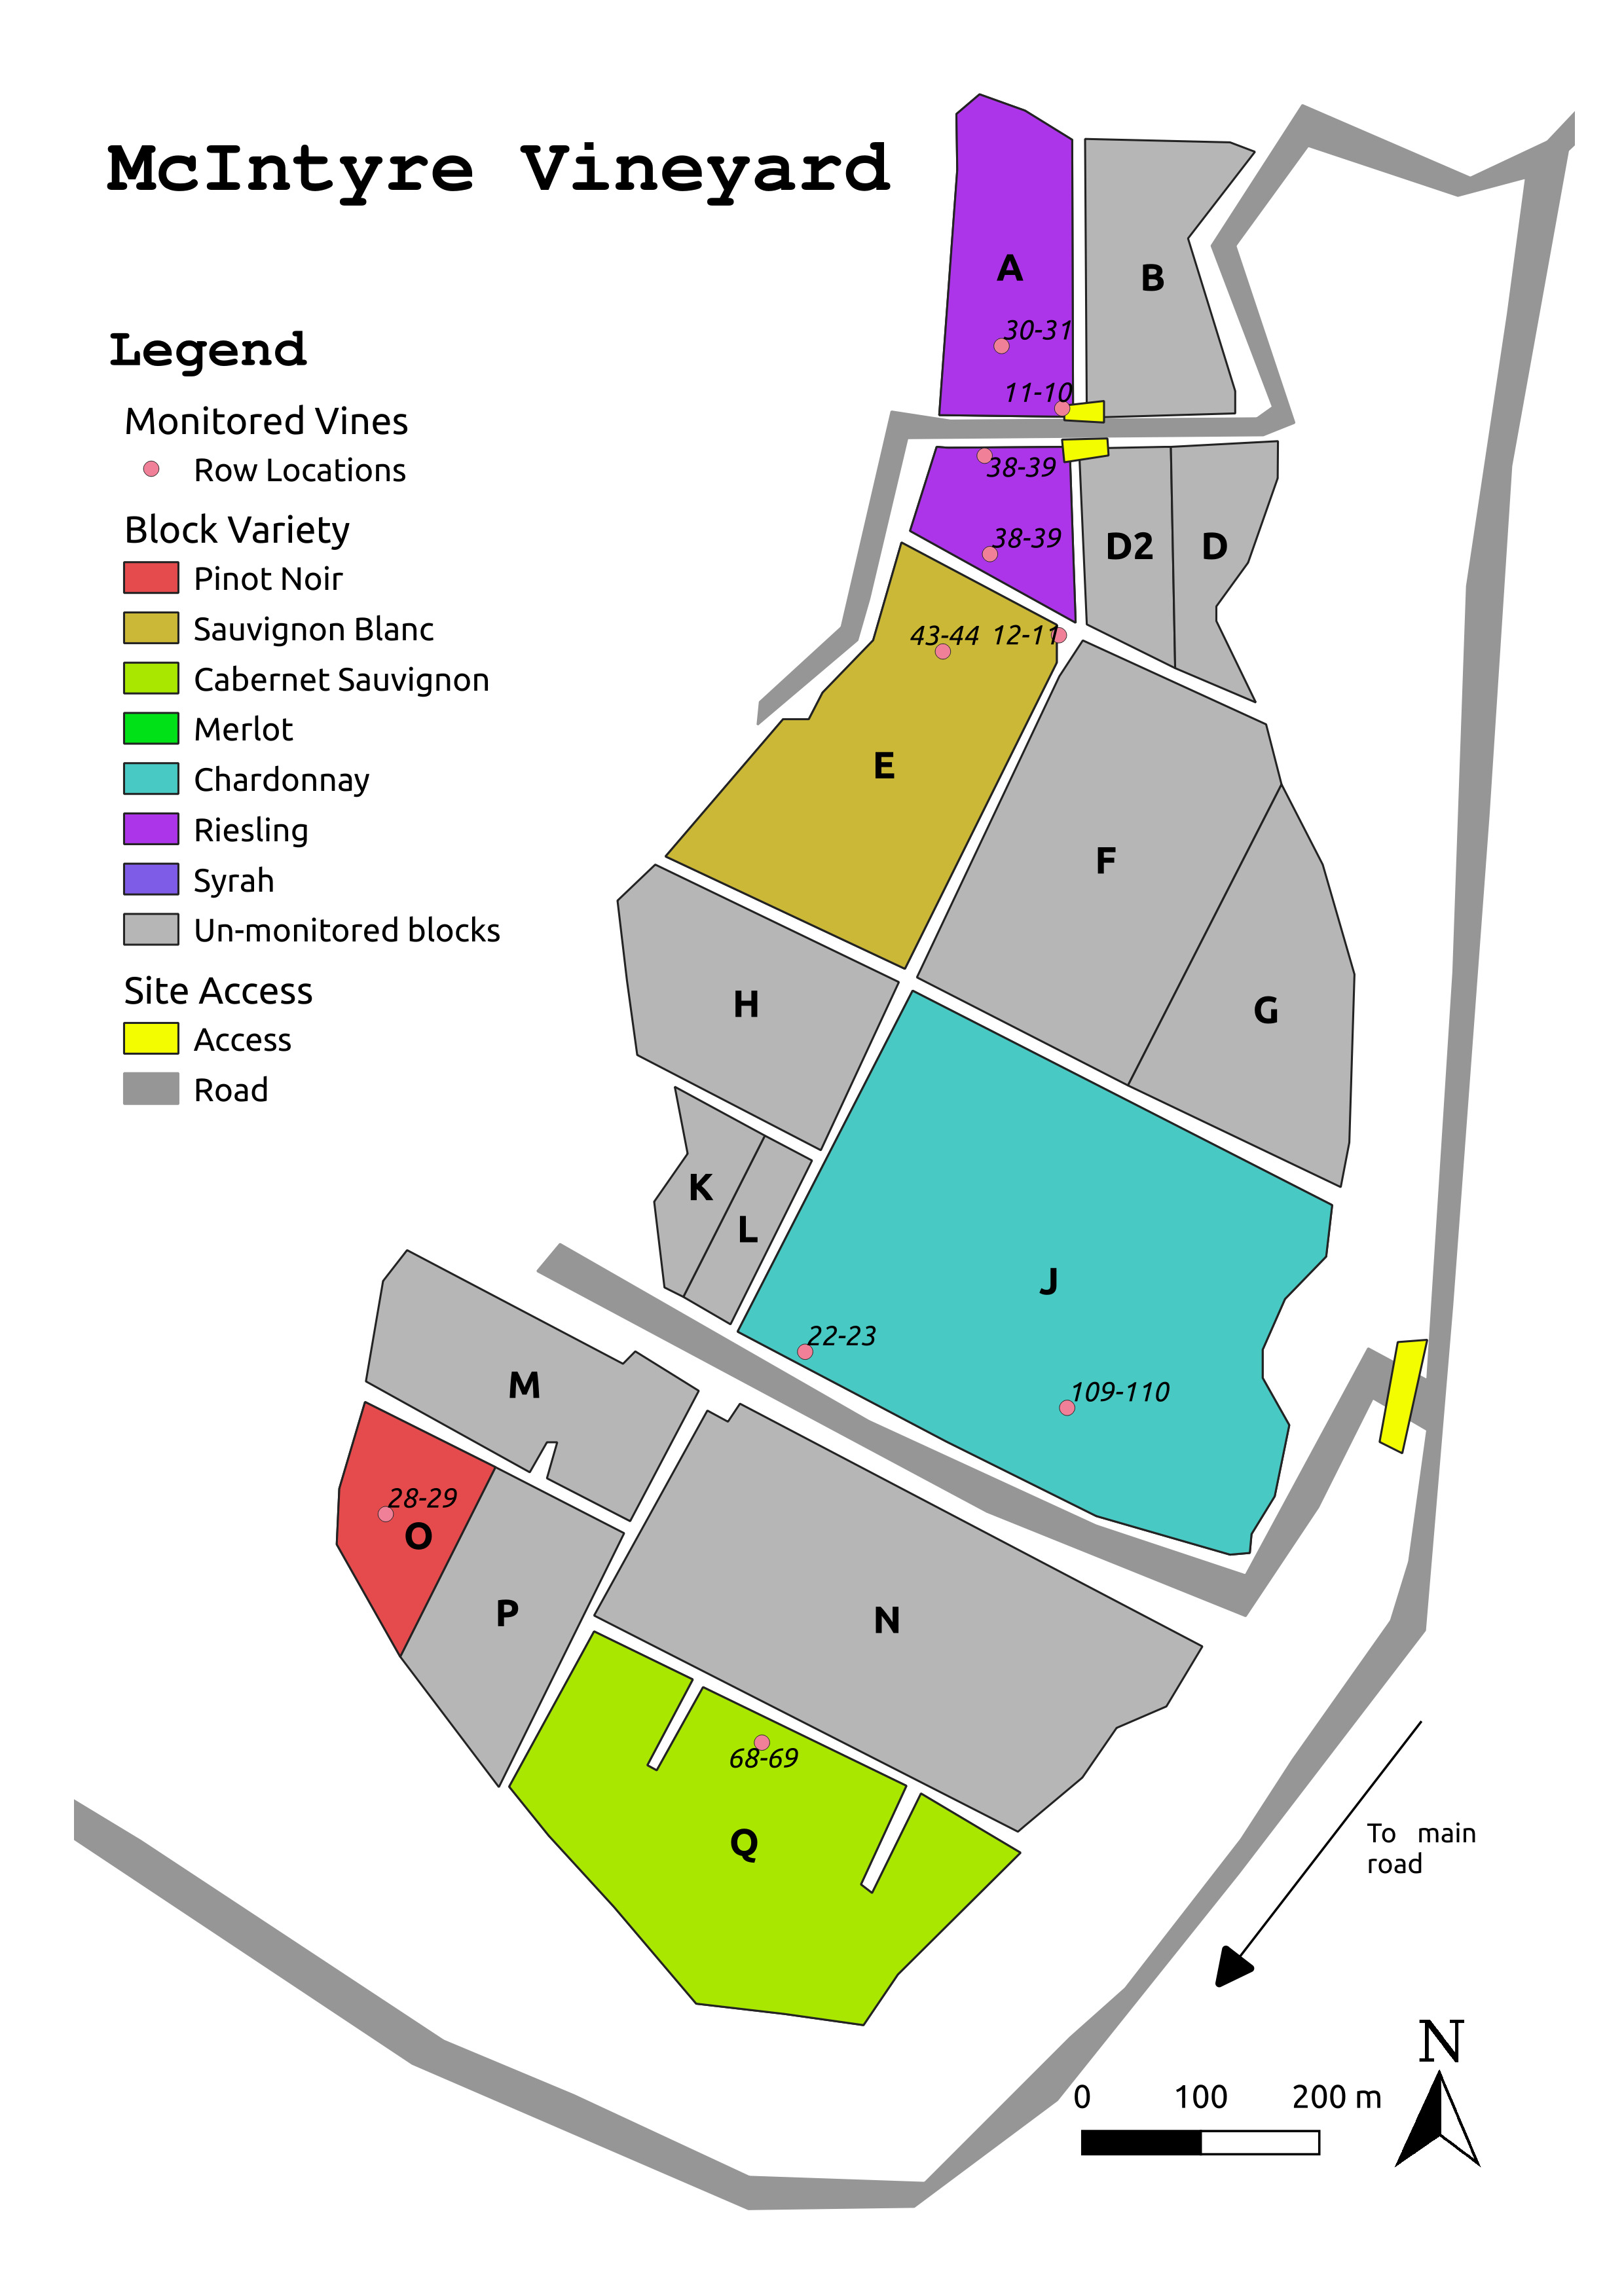
\includegraphics[width = \linewidth]{MC_Map.jpg}
  \caption{Map of McIntyre Vineyard}
  \label{fig:MCmap}
\end{figure}

\begin{figure} [h]
   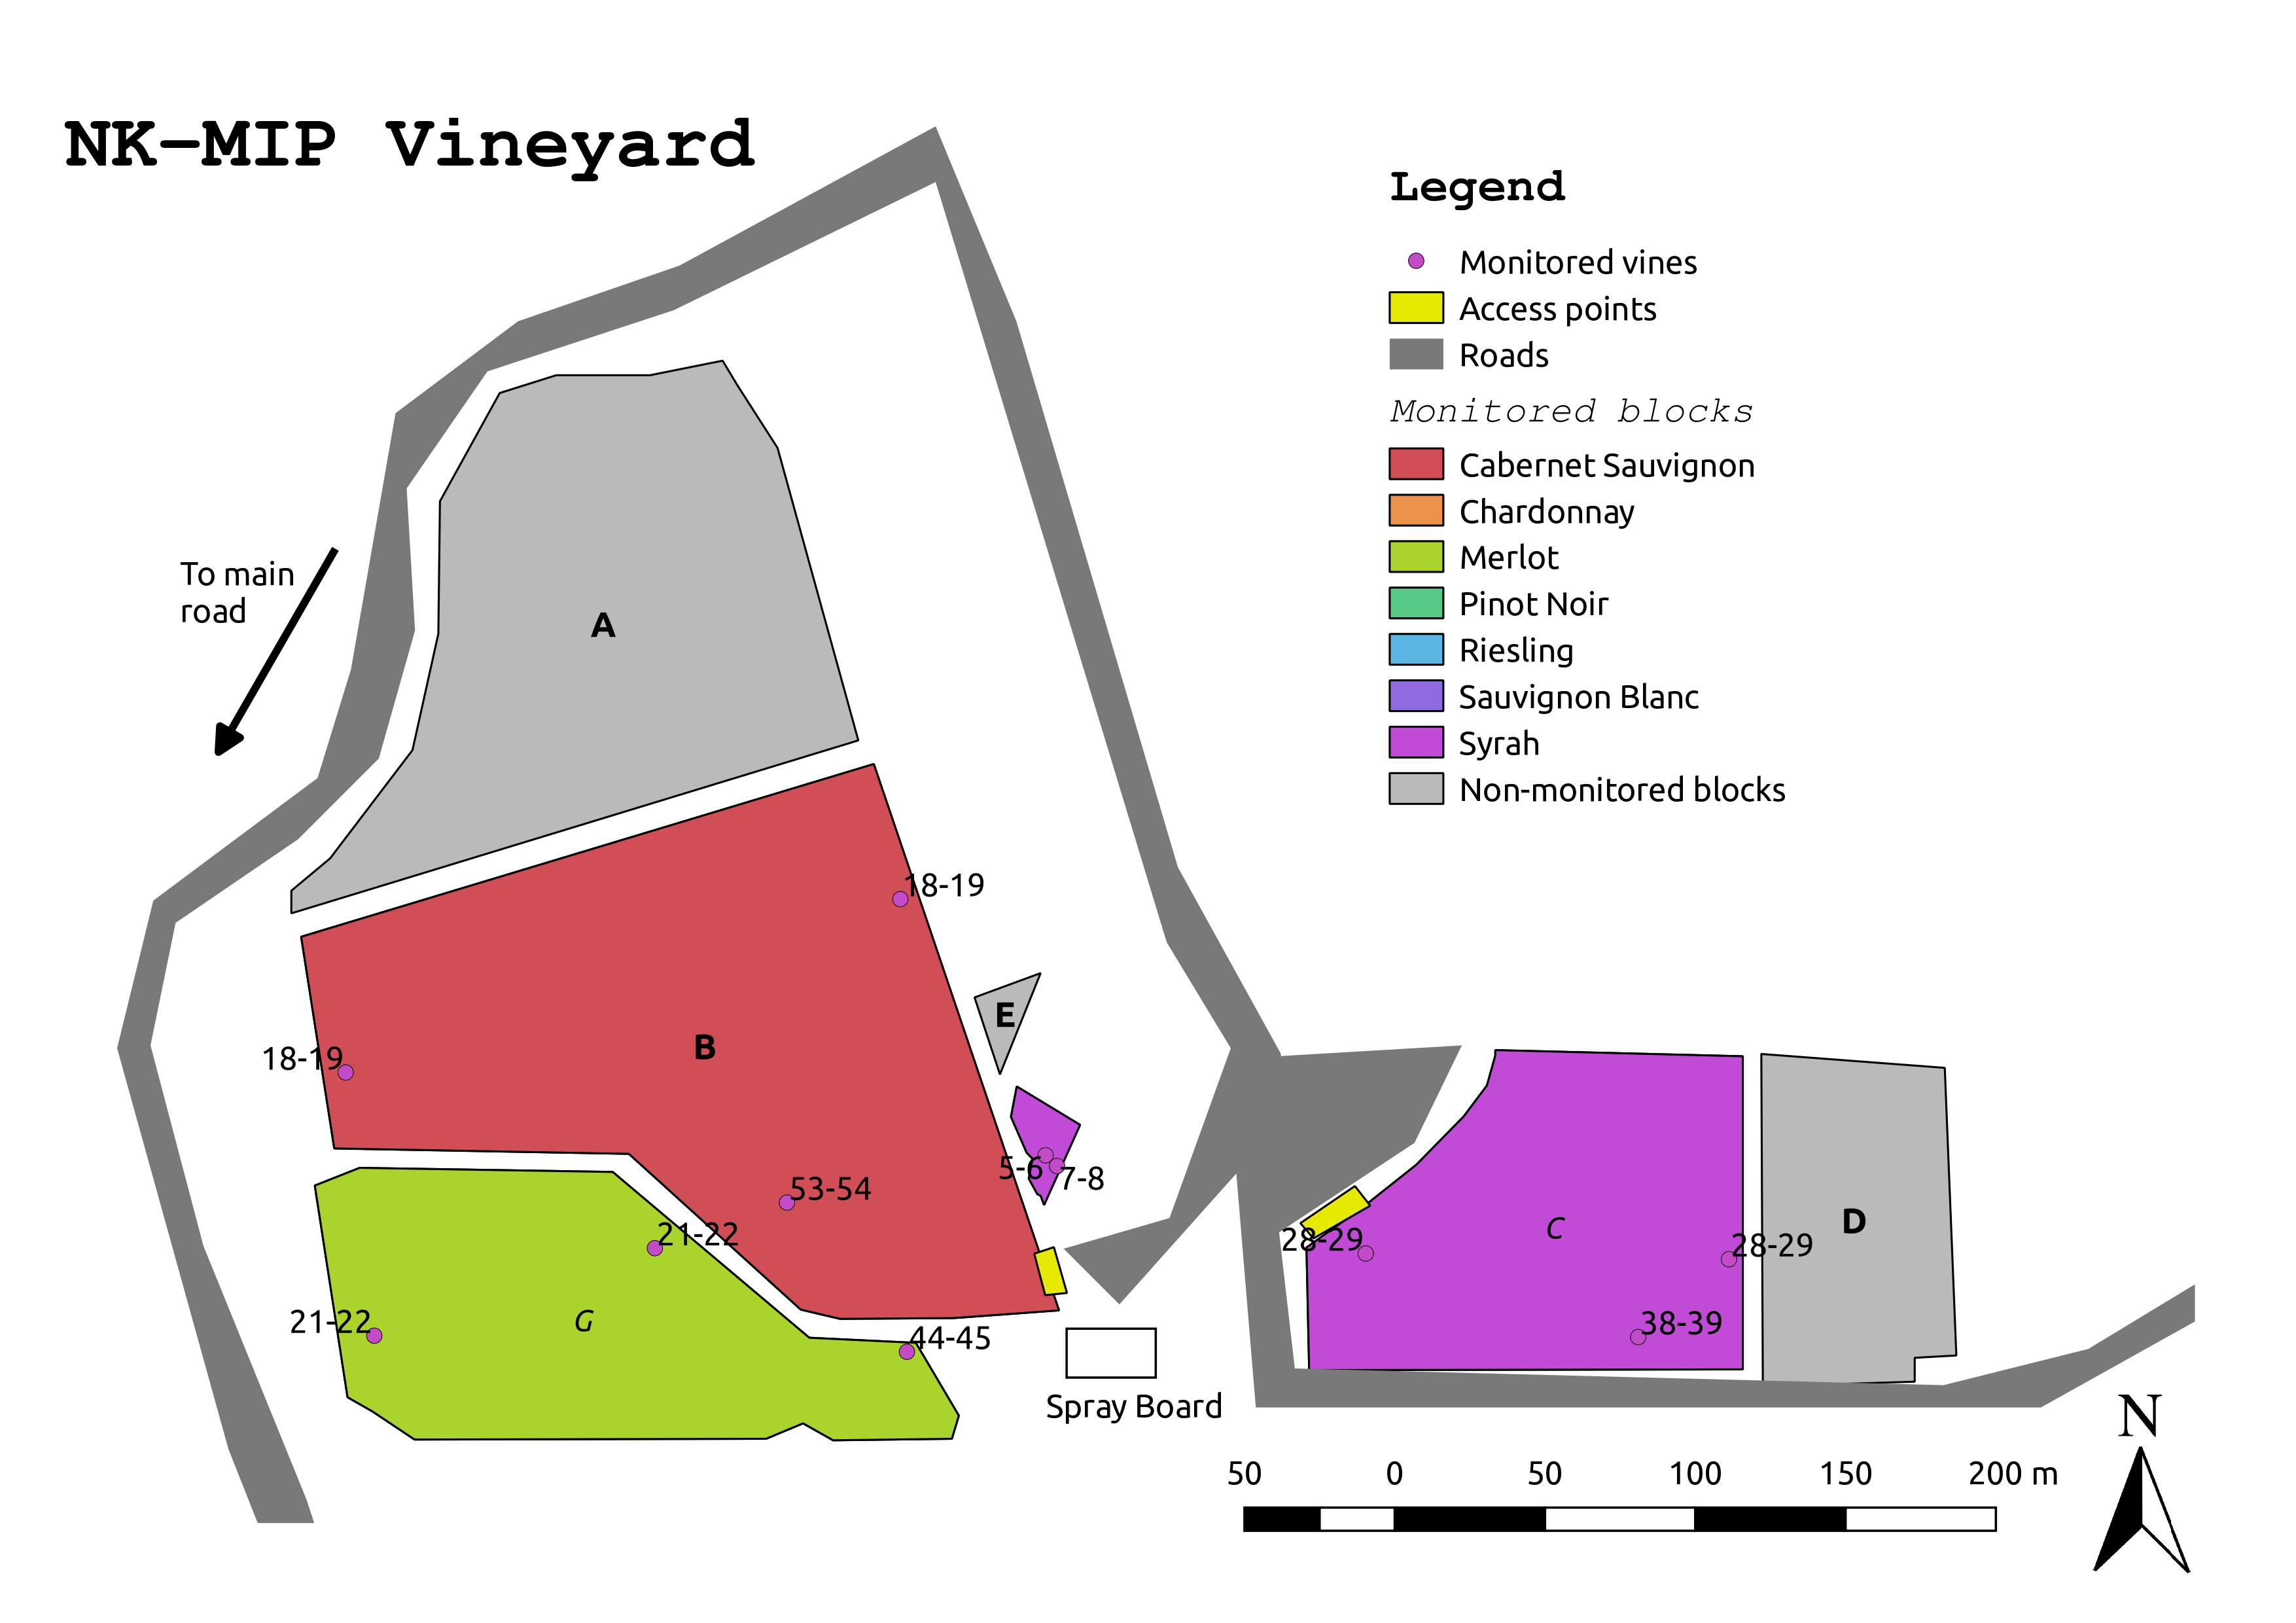
\includegraphics[width = \linewidth]{NK_Map.jpg}
  \caption{Map of Nk'Mip Cellars Vineyard}
  \label{fig:NKmap}
\end{figure}

\begin{figure} [h]
   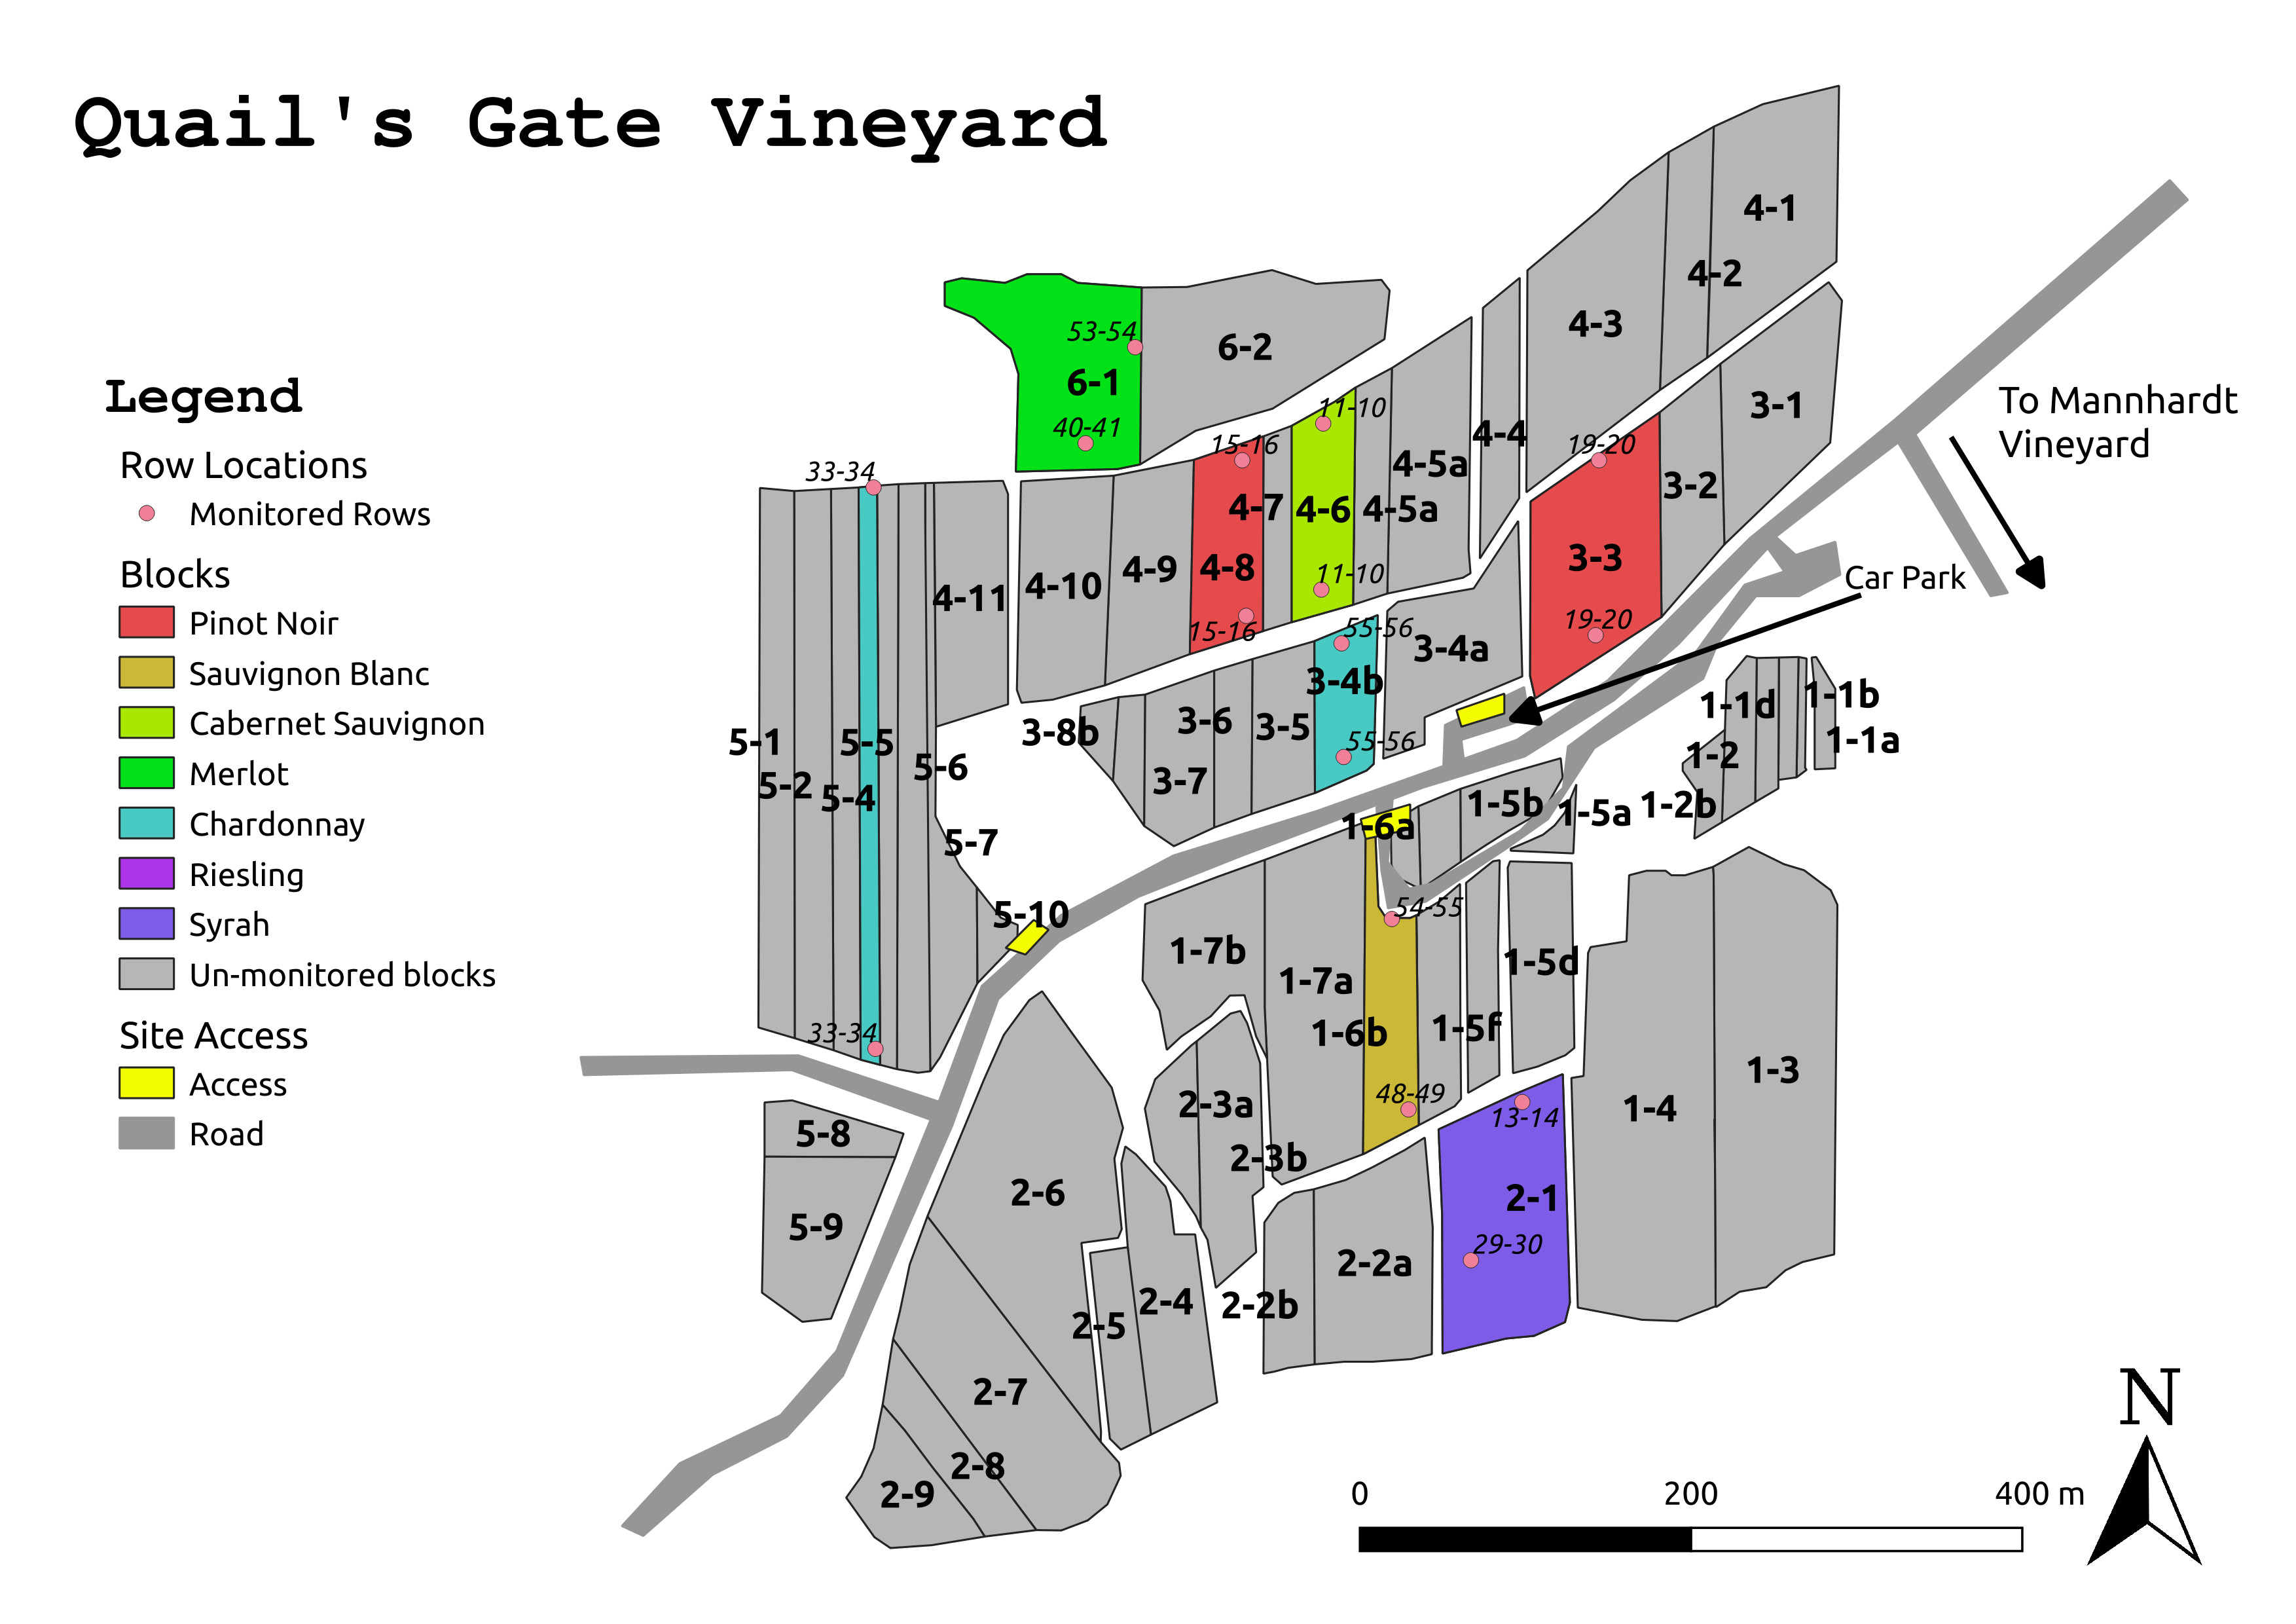
\includegraphics[width = \linewidth]{QG_Map.jpg}
  \caption{Map of Quails' Gate Estate Vineyard}
  \label{fig:QGmap}
\end{figure}

\begin{figure} [h]
   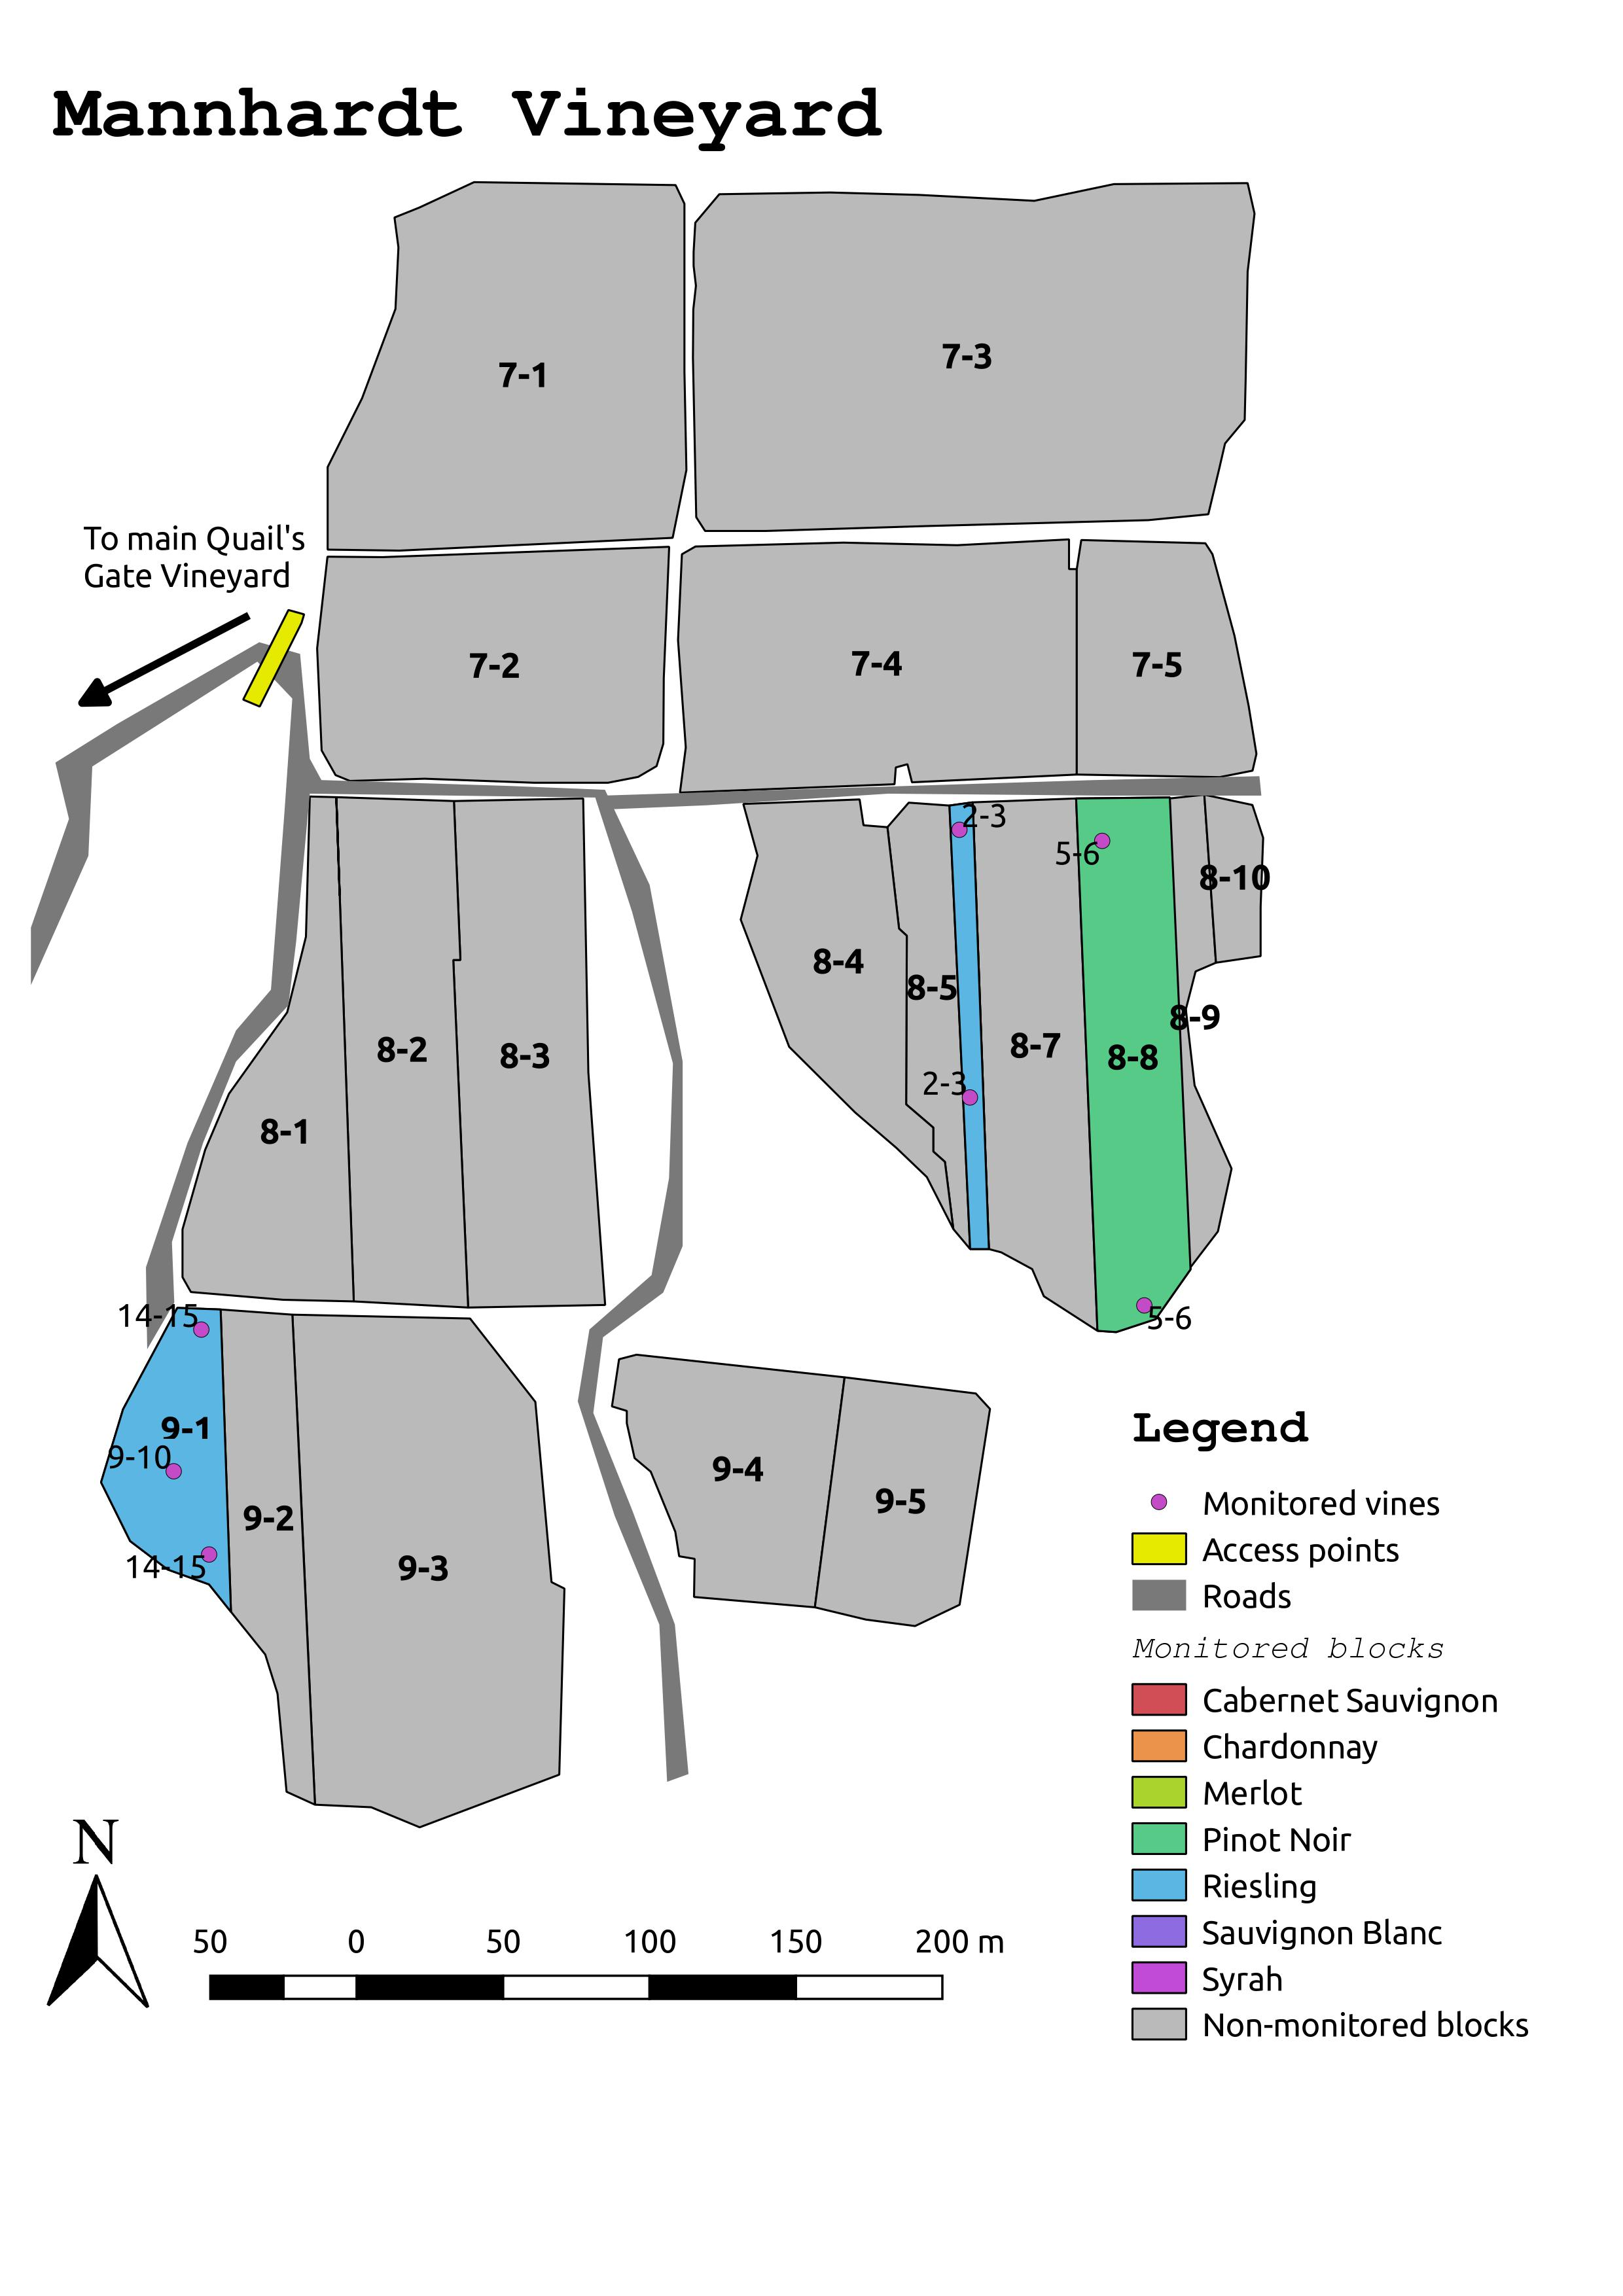
\includegraphics[width = \linewidth]{MA_Map.jpg}
  \caption{Map of Mannhardt Vineyard}
  \label{fig:MAmap}
\end{figure}


\end{document}

